\documentclass[
  aps,
  prb,
  preprint,
  superscriptaddress,
  longbibliography,
  nofootinbib
]{revtex4-2}

\usepackage[T1]{fontenc}
\usepackage[utf8]{inputenc}
\usepackage{amsmath,amssymb,bm}
\usepackage{mathtools}
\usepackage{dsfont}
\usepackage{booktabs}
\usepackage{graphicx}
\usepackage{microtype}
\usepackage{xcolor}
\usepackage{xr-hyper}
\externaldocument[SM-]{supplement}
\usepackage[colorlinks=true,allcolors=blue!45!black]{hyperref}

\newcommand{\dd}{\mathrm{d}}
\newcommand{\ee}{\mathrm{e}}
\newcommand{\ii}{\mathrm{i}}
\newcommand{\Tr}{\operatorname{Tr}}
\newcommand{\avg}[1]{\left\langle #1 \right\rangle}
\newcommand{\bR}{\mathbf{R}}
\newcommand{\br}{\mathbf{r}}
\newcommand{\bk}{\mathbf{k}}
\newcommand{\bp}{\mathbf{p}}
\newcommand{\bv}{\mathbf{v}}
\newcommand{\bnabla}{\boldsymbol{\nabla}}
\newcommand{\vF}{v_{\mathrm{F}}}
\newcommand{\vg}{v_{\mathrm{g}}}
\newcommand{\tautr}{\tau_{\mathrm{tr}}}
\newcommand{\elltr}{\ell_{\mathrm{tr}}}
\newcommand{\DOS}{N_1}
\newcommand{\DN}{D_{\mathrm{N}}}
\newcommand{\DE}{D(E)}
\newcommand{\LD}{L_D}
\newcommand{\Icoll}{I_{\mathrm{coll}}}
\newcommand{\fL}{f_L}
\newcommand{\fT}{f_T}
\newcommand{\qp}{\mathrm{qp}}
% --- merged in for the unified document (derivation-only macros + cleveref) ---
\usepackage[capitalize]{cleveref}
\crefname{equation}{Eq.}{Eqs.}
\Crefname{equation}{Eq.}{Eqs.}
\crefname{table}{Table}{Tables}
\Crefname{table}{Table}{Tables}
\crefname{section}{Sec.}{Secs.}
\Crefname{section}{Sec.}{Secs.}
\crefname{subsection}{Sec.}{Secs.}
\Crefname{subsection}{Sec.}{Secs.}
\crefname{subsubsection}{Sec.}{Secs.}
\Crefname{subsubsection}{Sec.}{Secs.}
\newcommand{\bA}{\mathbf{A}}
\newcommand{\bF}{\mathbf{F}}
\newcommand{\bH}{\mathbf{H}}
\newcommand{\bps}{\mathbf{p}_{\mathrm{s}}}
\newcommand{\bvg}{\mathbf{v}_{\mathrm{g}}}
\newcommand{\Iqp}{I_{\mathrm{qp}}}
\newcommand{\hatg}{\hat{g}}
\newcommand{\checkg}{\check{g}}
\newcommand{\hatD}{\hat{\Delta}}
\providecommand{\openone}{}\renewcommand{\openone}{\mathds{1}}
\newcommand{\Real}{\operatorname{Re}}
\newcommand{\Imag}{\operatorname{Im}}

\begin{document}

\title{Which Diffusion Equation for Nonequilibrium Superconducting Quasiparticles?}

\author{Soren Ormseth}
\affiliation{Department of Physics, University of Wisconsin--Madison, Madison, Wisconsin 53706, USA}

\date{\today}

\begin{abstract}
Spatially resolved modeling of nonequilibrium quasiparticles in
superconducting devices requires an energy-resolved diffusion equation,
and the literature reaches one by two apparently different routes:
projecting the quasiclassical kinetic theory onto a positive-energy
quasiparticle occupation and adding elastic impurity scattering to the
resulting Boltzmann-like equation, or taking the dirty limit at the
matrix (Usadel) level and reducing its Keldysh block. We compare the two
constructions in a common, explicitly delimited sector: a homogeneous
material, local BCS spectrum, isotropic \(s\)-wave gap, nonmagnetic Born
impurities, and no charge imbalance. The scalar route is shown to be an exact change of
variables of the dirty two-mode (Kopnin) reduction: the first angular
harmonic of the branch-projected occupation is the current-carrying
anisotropic transverse amplitude in disguise, and the coherence factors
of the impurity kernel force the transport-time closure
\(\tautr(E)=\DOS(E)\,\tau_{\mathrm N}\), equivalently
\(\DOS\,\DE=\DN\). Both routes then give the same operator, with
conserved spectral density \(\DOS f\), spatial spectral current
\(-\DN\bnabla_{\br}f\) undressed above the local gap edge and blocked
below it, and no density-of-states-gradient drift; the squared-DOS
dressing \(\DOS^2\) belongs to the transverse charge-imbalance channel.
What does differ, measurably, is the legacy operator placement
\(\bnabla\cdot[(\DN/\DOS)\bnabla f]\)---the form in common use in
device modeling, including as the energy-resolved starting point of
published analyses of gap-engineered quasiparticle traps: it treats
the occupation itself as the conserved density and acquires a spurious
DOS-gradient drift once the gap is inhomogeneous---as it always is, at
some amplitude, once the occupation feeds back on the gap. We organize the
candidate operators into a two-exponent family \(L_{p,q}\), derive the
Kupriyanov--Lukichev interface condition for the scalar current, and
benchmark the operators numerically on prescribed and self-consistently
generated gap profiles; under the legacy placement quasiparticles drift
into the gap well their own population digs, whereas the microscopic
operator predicts no such self-focusing. We delimit the assumptions
behind the equivalence and the regimes in which the two-mode or matrix
equations must be retained instead.
\end{abstract}

\maketitle

% ===================== BODY (from main.tex) =====================

\section{Introduction}
Spatially resolved modeling of nonequilibrium quasiparticles in
superconducting devices turns on a question that sounds innocuous:
which energy-resolved spatial operator \(\LD\) moves the quasiparticle
occupation \(f(E,\br,t)\) through the device? Recent resonator and
qubit treatments are usually spatially homogeneous or zero-dimensional
in their kinetics
\cite{goldie2013,catelani2019,fischer2023,fischer2024,marchegiani2025},
but spatial simulations---normal-metal and gap-engineered
quasiparticle traps are the prototypical examples
\cite{riwar2016,hosseinkhani2018,riwar2019}---cannot avoid the choice,
and the published equations differ in form. Normal-metal-trap analyses
diffuse the energy-integrated density with a constant coefficient
\cite{riwar2016,hosseinkhani2018}; the gap-engineered-trap analysis of
Ref.~\onlinecite{riwar2019} starts instead from the energy-resolved
coefficient \(\DN/\DOS(E)\)---\(\DN\) the normal-state diffusion
constant, \(\DOS\) the BCS density-of-states factor---placed inside
the divergence, \(\bnabla_{\br}\cdot[(\DN/\DOS)\bnabla_{\br}f]\), a
Fick ansatz for the occupation itself.

For a spatially uniform gap the choice is invisible. The coefficient
\(\DN/\DOS(E)\) is microscopically supported---the
Bardeen--Rickayzen--Tewordt coherence-factor cancellation produces
exactly this rate \cite{bardeen1959}---and every placement of the
spectral weight \(1/\DOS\) yields the same uniform-gap relaxation.
Once \(\Delta\) varies in space, the placements separate measurably:
at fixed energy the density of states varies with position, and the
Fick placement acquires a density-of-states-gradient drift, divergent
toward the local gap edge, that drives quasiparticles down the gap
gradient---into an engineered gap well, and into the well that a
localized population digs for itself through the self-consistent
gap---whereas the microscopically selected operator carries no such
drift at any amplitude. Spatial gap variation is not an exotic
circumstance: it is engineered deliberately in traps and generated
dynamically by any nonuniform population, so the distinction is
engaged, at some amplitude, in every self-consistent spatial device
model.

This paper settles the placement from the microscopic theory, by both
routes the literature uses to reach an energy-resolved kinetic
equation: projecting the quasiclassical theory onto a positive-energy
quasiparticle occupation and adding elastic impurity scattering to the
resulting Boltzmann-like equation, or angular averaging the matrix
theory into the Usadel equation and reducing its Keldysh block. Within
a common, explicitly delimited sector---homogeneous material, local
BCS spectra, isotropic \(s\)-wave gap, nonmagnetic Born impurities,
negligible charge imbalance---the two routes select the \emph{same}
operator: conserved spectral density \(\DOS f\), spatial current
\(-\DN\bnabla_{\br}f\) undressed above the local gap edge and blocked
below it, and no density-of-states-gradient drift---the operator
labeled A1 in the taxonomy of \cref{sec:taxonomy}---with the
squared-DOS dressing \(\DOS^{2}\) belonging to the transverse
(charge-imbalance) channel. The candidate placements are organized
into a two-exponent operator family \(L_{p,q}\), the
Kupriyanov--Lukichev interface condition is projected onto the same
scalar current, and the operators are benchmarked numerically on
prescribed and self-consistently generated gap profiles
(\cref{sec:program}). The remainder of this introduction assembles the
quasiclassical machinery from which both routes start.

The Eilenberger equation for superconductors is derived from the
Gor'kov (Nambu--Keldysh) Green-function equations of motion under the
quasiclassical approximation
\cite{eilenberger1968,eliashberg1972,larkin1986,rammer1986,kopnin2001}:
all energies characterizing the superconducting state and its dynamics
(\(\Delta\), \(k_{\mathrm B}T\), \(\hbar\omega\), \(\hbar/\tau\)) are taken small
compared with the Fermi energy. Equivalently, all relevant lengths
(the coherence length \(\xi_0\), the mean free path \(\elltr\), and
the scales on which \(\Delta\) varies) are long compared with the
Fermi wavelength. These assumptions mean that the propagator is sharply peaked at the
Fermi surface, and the self-energy splits into a coherent mean-field
part and a collision part. For the singlet BCS model considered here the
anomalous mean-field self-energy is absorbed into the gap matrix
\(\hatD\), while any diagonal coherent shifts are taken to have been
absorbed into the quasiparticle energy or external potentials. The
remaining collision self-energy
\(\check{\Sigma}_{\mathrm{coll}}=\check{\Sigma}_{\mathrm{imp}}+\check{\Sigma}_{\mathrm{inel}}\)
collects elastic impurity scattering together with inelastic processes
such as electron--phonon scattering and photon absorption or emission
represented through an effective self-energy. The Eilenberger equation is obtained from the Wigner-transformed
Dyson equation, gradient-expanded to first order in the slow
center-of-mass variables: the difference of the left- and
right-acting equations is integrated over the normal-state
quasiparticle energy \(\xi_{\bk}\), removing the fast momentum
dependence. The result is a transport equation for the
trajectory-resolved quasiclassical propagator
\(\checkg(E,\hat{\bp},\br,t)\),
\begin{equation}
  \hbar\vF\,\hat{\bp}\cdot\widetilde{\bnabla}_{\br}\,\checkg
  +
  \ii\bigl[\,E\tau_3-\hatD-\check{\Sigma}_{\mathrm{coll}},\;\checkg\,\bigr]_{\otimes}
  =
  0,
  \qquad
  \checkg\otimes\checkg=\openone,
  \label{eq:intro_eilenberger}
\end{equation}
where \(\widetilde{\bnabla}\) is the gauge-covariant gradient,
\(\hatD=-\ii\Delta\tau_2\) is the gap matrix in the gauge of real
\(\Delta\), and \(\otimes\) denotes the convolution over internal time
(Wigner energy) arguments.
In this gauge the coherent generator
\(E\tau_3-\hatD=E\tau_3+\ii\Delta\tau_2\) squares to
\((E^{2}-\Delta^{2})\openone\) and is proportional to the BCS retarded
propagator on the spectral branch, fixing the gapped spectrum. The
overall factor \(\ii\) multiplying the commutator balances the real
streaming term.
The normalization \(\checkg\otimes\checkg=\openone\) closes the
transport problem and selects the physical solution manifold.

Because \(\checkg\) carries the full Keldysh structure,
\cref{eq:intro_eilenberger} actually packages three coupled equations:
its retarded and advanced blocks are Eilenberger's spectral equations
\cite{eilenberger1968}, which in the homogeneous weak-coupling limit fix
the BCS density of states and coherence factors, while its Keldysh block
is the Eliashberg equation \cite{eliashberg1972,larkin1986}, which
governs the nonequilibrium distribution. The kinetic equation derived
below is built on this Keldysh (Eliashberg) component. In the
approximation used below, the spectral and kinetic blocks decouple and
can be solved separately.
The validity of this relies on an adiabatic local-BCS
spectral approximation, in which the retarded and advanced propagators are
taken to have their equilibrium BCS form evaluated at the instantaneous
local gap, and the gap-driven
spectrum varies slowly enough to track quasi-statically
(\(\hbar|\xi_{\bk}\dot\Delta|/E^3\ll1\)). The distribution still feeds back on the spectrum, but only
through the gap: the self-consistent \(\Delta\) responds to the
occupation, and the spectrum follows. What the closure drops is the
\emph{direct} channel, in which the nonequilibrium distribution would
dress the retarded and advanced propagators through the collision
self-energy---broadening, shifting, or damping the density of states
and coherence factors independently of \(\Delta\). What remains to be determined then is the evolution of the nonequilibrium distribution at a fixed,
gap-determined spectrum.
\subsection{Quasiparticle Kinetic Equations}
Throughout, we reserve \(f\)-type symbols for quasiparticle
distribution functions (with \(f\) an occupation probability but
\(\fL,\fT\) distribution amplitudes) and \(n\) for phonon occupations.
One further distinction is worth posting in advance, because readers
coming from branch-resolved treatments often elide it: Kopnin's
transverse amplitude is the spectrally \emph{weighted} branch-odd
combination \(\fT=\lambda_{\bk}\phi_T\)---an identity for the
\emph{even} angular harmonics only; the odd harmonics swap sectors,
\cref{eq:intro_parity_dictionary}---with \(\lambda_{\bk}\) the
spectral weight of \cref{eq:beta_sigma_lambda}, not the bare branch
difference \(\phi_T\); the two are kept carefully distinct from
\cref{eq:intro_branch_traj} onward.

The quasiparticle content is carried by two scalar modes, the
longitudinal (energy) mode \(\fL\) and the transverse (charge-imbalance)
mode \(\fT\). In the electron--hole (Nambu) basis, with
\(\tau_3=\operatorname{diag}(+1,-1)\), the diagonal distribution matrix is
\begin{equation}
  \hat h
  = \fL\,\openone + \fT\,\tau_3
  = \begin{pmatrix} \fL+\fT & 0\\[2pt] 0 & \fL-\fT \end{pmatrix}
  \label{eq:intro_h_matrix}
\end{equation}
[Kopnin's \(f^{(1)}=\fL\), \(f^{(2)}=\fT\), Eqs.~(10.33)--(10.34) of
Ref.~\onlinecite{kopnin2001}; see also Ref.~\onlinecite{schmidschon1975}].
Its diagonal entries \(\fL\pm\fT\) are the particle and hole amplitudes,
so \(\fL\) is their symmetric part and \(\fT\) their antisymmetric part;
inverting \cref{eq:intro_h_matrix},
\begin{equation}
  \fL = \tfrac12\Tr\hat h,
  \qquad
  \fT = \tfrac12\Tr[\tau_3\hat h]
      = \tfrac12\bigl[(\fL+\fT)-(\fL-\fT)\bigr],
  \label{eq:intro_fLfT_traces}
\end{equation}
which fixes the sign of \(\fT\) (even in \(E\)). A positive \(\fT\)
counts an excess of hole-like over electron-like quasiparticles---the
charge imbalance \cite{tinkham2004}---and enters the electron density
through \(\delta N=-N_0\!\int\!\langle\DOS\,\fT\rangle\,\dd E\)
[Kopnin's Eqs.~(10.69)--(10.71)], with
\(N_0=m p_{\mathrm F}/2\pi^2\hbar^3\) the single-spin normal-state
density of states at the Fermi level---Kopnin's \(\nu(0)\), whose
definition fixes the same single-spin normalization
\cite{kopnin2001}---used for this quantity throughout, fixing the sign
independent of the branch labelling. When both branches share a common quasiparticle
occupation \(f\), then \(\fT=0\) and \(\fL=1-2f\).

Kopnin has shown \cite[\S10.2]{kopnin2001} that, after parametrizing
the Keldysh propagator with the two-mode distribution matrix
\(\hat h=\fL\,\openone+\fT\,\tau_3\) introduced above and projecting the
\(\xi_{\bk}\)-integrated transport equation onto its scalar
\(\openone\)- and \(\tau_3\)-traces, the nonequilibrium (Eliashberg) block
reduces to a coupled pair of \emph{two-mode} scalar kinetic equations
for \(\fL\) and \(\fT\) [his Eqs.~(10.41) and~(10.44)]. Standard
Eilenberger ordering drops the augmented \((k_F\xi_0)^{-1}\)
momentum-derivative forces; because one of the questions below is how the
ballistic and dirty reductions compare when such gradient terms are
retained, we keep the leading pair-potential-gradient contribution
explicitly as \(\mathcal{R}[\fL]\). Specialized to the sector of interest
here---real gap, no superflow, no electric field, continuum energies
\(E>\Delta\), and before any angular averaging---this parent pair reads
\begin{align}
  \DOS\,\partial_t\fL
  + N_2\,\dot\Delta\,\partial_E\fL^{(0)}
  + \vF\,\hat{\bp}\cdot\bnabla_{\br}\!\left(\DOS\,\fT\right)
  + \mathcal{R}[\fL]
  &= J_L,
  \label{eq:beta_twomode_L}\\
  \DOS\,\vF\,\hat{\bp}\cdot\bnabla_{\br}\,\fL
  &= J_T,
  \label{eq:beta_twomode_T}
\end{align}
where the local BCS spectral functions are
\begin{equation}
  \DOS(E)=\frac{E}{\Omega},\qquad
  N_2(E)=\frac{\Delta}{\Omega},\qquad
  \Omega(E,\br,t)=\sqrt{E^{2}-\Delta^{2}(\br,t)},
  \label{eq:beta_spectral}
\end{equation}
\(\fL^{(0)}=\tanh(E/2k_{\mathrm B}T)\) is the equilibrium longitudinal
amplitude, and \(J_L,J_T\) are the \(\openone\)- and
\(\tau_3\)-projections of the Keldysh source terms---collision
self-energies and, in the transverse sector, the coherent gap-mediated
conversion terms where present. The term
\(\mathcal{R}[\fL]\) collects the momentum-derivative forces of Kopnin's
Eq.~(10.41): the Lorentz force, which is absent here as we carry no
fields, and the pair-potential-gradient (refraction) force, which for an
isotropic gap reduces to a single term \(\propto
N_2\,(\widetilde{\bnabla}_{\br}\Delta)\) acting on the
trajectory-angular derivative of \(\fL\).

The explicit \(N_2\,\dot\Delta\,\partial_E\fL^{(0)}\) source is Kopnin's
linearization about local equilibrium; in the positive-energy Boltzmann
rewriting below the same adiabatic spectral-flow physics is promoted to
the convective derivative \(\tfrac{\Delta}{E}\dot\Delta\,\partial_E\)
acting on the full distribution amplitude.

The source terms \(J_L,J_T\) are projections of the full Keldysh source
structure, and so the scattering physics---elastic impurity,
electron--phonon, and the rest---is contained in them. From this point one
can specialize to either the clean or the dirty limit, and the fork turns
on how the parent equations carry the spatial current: it flows through
the transverse amplitude \(\fT\)---the \(\bnabla_{\br}(\DOS\,\fT)\) term,
not \(\fL\) directly---with \cref{eq:beta_twomode_T} slaving the
anisotropic part of \(\fT\) to \(\bnabla_{\br}\fL\), the structure the
dirty route isotropizes into diffusion. The clean route may instead retain
\(\mathcal{R}[\fL]\) at augmented-clean quasiclassical order---legitimate
while \(|\Delta|\) and any supercurrent are nearly uniform---recombining
the two modes without eliminating any harmonic before the refraction force
is dropped at standard Eilenberger order (next subsection).

\subsection{Quasiparticle Boltzmann-Like Equations}
We now recombine the two-mode pair
\cref{eq:beta_twomode_L,eq:beta_twomode_T} into a single Boltzmann-like
equation. We assume only that the
spectral problem is local enough that quasiparticles carry a positive
semiclassical energy \cite[\S15.2]{kopnin2001}. The
branch occupation is a momentum-space object, so we work in the momentum
direction \(\hat{\bk}\); the trajectory-resolved amplitudes
\(\fL,\fT\) of \cref{eq:beta_twomode_L,eq:beta_twomode_T} enter in their
momentum-direction representation, related by the branch relabelling
\(\hat{\bp}=\sigma\hat{\bk}\) below.

With fields present it is the gauge-invariant transverse mode that
appears,
\begin{equation}
  \fT' = \fT - e\Phi\,\partial_E\fL^{(0)},
  \qquad
  \Phi = \varphi + \frac{\hbar}{2e}\,\partial_t\chi,
  \label{eq:beta_fT_shift}
\end{equation}
together with the gauge-invariant superfluid momentum
\begin{equation}
  \bps = \frac12\!\left(\hbar\bnabla\chi - \frac{2e}{c}\bA\right).
  \label{eq:beta_ps_def}
\end{equation}
In the local-quasiparticle approximation the branch energy is
\begin{equation}
  \varepsilon_{\bk} = \widetilde E_{\bk} + \bps\cdot\vF\hat{\bk},
  \qquad
  \widetilde E_{\bk} = \sqrt{\widetilde\xi_{\bk}^{\,2}+|\Delta|^2},
  \qquad
  \widetilde\xi_{\bk} = \xi_{\bk} + e\Phi ,
  \label{eq:beta_qp_energy}
\end{equation}
and, with the branch label and BCS velocity factor
\begin{equation}
  \sigma \equiv \operatorname{sgn}\widetilde\xi_{\bk} = \pm1,
  \qquad
  \lambda_{\bk} \equiv \frac{|\widetilde\xi_{\bk}|}{\widetilde E_{\bk}},
  \label{eq:beta_sigma_lambda}
\end{equation}
the group velocity is
\begin{equation}
  \bvg \equiv \hbar^{-1}\partial_{\bk}\varepsilon_{\bk}
  = \frac{\widetilde\xi_{\bk}}{\widetilde E_{\bk}}\,\vF\hat{\bk}
  = \sigma\lambda_{\bk}\,\vF\hat{\bk}.
  \label{eq:beta_group_velocity}
\end{equation}

The crucial step passes from the two amplitudes \(\fL,\fT'\) to the
positive-energy occupation \(f_{\bk}\), equivalently
\(h_{\bk}\equiv1-2f_{\bk}\). In the quasiparticle-occupation convention used throughout---both
branches carrying \(f(E)\) in equilibrium---the branch distribution is
[equivalent to Kopnin's Eq.~(15.4) with the hole branch's occupation
conjugated]
\begin{equation}
  h_{\bk}
  = \fL + \sigma\,\lambda_{\bk}^{-1}\,\fT',
  \qquad\text{i.e.}\qquad
  f_{\bk}
  = \frac12\!\left[
    1 - \fL
    - \sigma\,\frac{\widetilde E_{\bk}}{|\widetilde\xi_{\bk}|}\,\fT'
  \right],
  \label{eq:beta_f_from_modes}
\end{equation}
with \(\sigma=\operatorname{sgn}\widetilde\xi_{\bk}\) and all amplitudes
evaluated at \((\varepsilon_{\bk},\hat{\bk},\br,t)\).
Explicitly, if \(n_{\bk}^{\mathrm K}\) denotes Kopnin's occupation [his
Eq.~(15.4)], whose equilibrium form is the Fermi function of
\(\varepsilon_{\bk}\) only on the electron-like branch, the conjugation
is the single line
\begin{equation}
  h_{\bk}
  \equiv 1-2f_{\bk}
  = \sigma\bigl(1-2n_{\bk}^{\mathrm K}\bigr)
  = f^{(1)}+\sigma\,\lambda_{\bk}^{-1}f_2' ,
  \label{eq:beta_conjugation_map}
\end{equation}
identifying \(\fL=f^{(1)}\) and \(\fT'=f_2'\): the branch sign
\(\sigma\) multiplies the longitudinal amplitude in Kopnin's convention
and the transverse one in ours, the two forms differing by the overall
factor \(\sigma\).
Writing \(h_\sigma\equiv1-2f_\sigma\) for the two signs of
\(\widetilde\xi_{\bk}\) at fixed \(\widetilde E_{\bk}\), the inverse is
\begin{align}
  \fL &= \tfrac12\textstyle\sum_{\sigma=\pm1}h_\sigma
       = \tfrac12(h_++h_-),
  \label{eq:beta_fL_inverse}\\
  \fT' &= \tfrac{\lambda_{\bk}}{2}\textstyle\sum_{\sigma=\pm1}\sigma\,h_\sigma
       = \tfrac{\lambda_{\bk}}{2}(h_+-h_-).
  \label{eq:beta_fT_inverse}
\end{align}
The longitudinal mode is thus the branch-even (symmetric) part of
\(h_\sigma\)---nonzero in equilibrium, \(\fL^{(0)}=\tanh(E/2k_{\mathrm
B}T)\)---and the (shifted) transverse mode the branch-odd part weighted
by \(\lambda_{\bk}\); the occupation \(f_{\bk}\) has no definite parity in
\(\widetilde\xi_{\bk}\), and the two-mode formulation is precisely its
parity decomposition. The relabelling \(\hat{\bp}=\sigma\hat{\bk}\) is
what carries the trajectory-resolved amplitudes of
\cref{eq:beta_twomode_L,eq:beta_twomode_T} into these momentum-direction
combinations.

The semiclassical motion is \(\dot\br=\bvg\) and
\begin{equation}
  \hbar\dot\bk = \bF_{\bk}
  = -\bnabla_{\br}\varepsilon_{\bk} + \bF_L,
  \qquad
  \bF_L = \frac{e}{c}\,\vF\hat{\bk}\times\bH,
  \label{eq:beta_pdot}
\end{equation}
with Liouville operator
\begin{equation}
  \mathcal L_{\bk}
  = \partial_t + \bvg\cdot\bnabla_{\br}
  + \frac{\bF_{\bk}}{\hbar}\cdot\partial_{\bk},
  \label{eq:beta_liouville}
\end{equation}
or, in variables \((E,\hat{\bk})\),
\begin{equation}
  \mathcal L_{\bk}
  = \partial_t + \dot E_{\bk}\,\partial_E
  + \bvg\cdot\bnabla_{\br} + \dot{\hat{\bk}}\cdot\bnabla_{\hat{\bk}},
  \qquad
  \dot E_{\bk} = \partial_t\varepsilon_{\bk},
  \quad
  \dot{\hat{\bk}}
  = \frac{(\openone-\hat{\bk}\hat{\bk})\cdot\bF_{\bk}}{\hbar k_F}.
  \label{eq:beta_liouville_energy_variables}
\end{equation}
The equality \(\dot E_{\bk}=\partial_t\varepsilon_{\bk}\) is the
Hamiltonian structure of the motion: along a trajectory
\(\dot\br\cdot\bnabla_\br\varepsilon_{\bk}
+\dot\bk\cdot\partial_{\bk}\varepsilon_{\bk}=0\)
(the Lorentz force is orthogonal to \(\bvg\)), so spatial forces
redistribute momentum without sourcing energy beyond the explicit time
dependence of the local spectrum. For zero superflow,
\begin{equation}
  \dot E_{\bk}
  = \frac{|\Delta|\,\partial_t|\Delta| + \widetilde\xi_{\bk}\,e\dot\Phi}
         {\widetilde E_{\bk}} .
  \label{eq:beta_Edot_simple}
\end{equation}

The Boltzmann-like equation is therefore
\begin{equation}
  \mathcal L_{\bk} f_{\bk} = \Iqp[f,n],
  \qquad\text{i.e.}\qquad
  \partial_t f_{\bk}
  + \bvg\cdot\bnabla_{\br}f_{\bk}
  + \frac{\bF_{\bk}}{\hbar}\cdot\partial_{\bk}f_{\bk}
  = \Iqp[f,n],
  \label{eq:beta_boltzmann_explicit}
\end{equation}
or, in the energy--angle representation,
\begin{equation}
  \partial_t f_{\bk}
  + \dot E_{\bk}\,\partial_E f_{\bk}
  + \bvg\cdot\bnabla_{\br}f_{\bk}
  + \dot{\hat{\bk}}\cdot\bnabla_{\hat{\bk}}f_{\bk}
  = \Iqp[f,n],
  \label{eq:beta_boltzmann_energy_variables}
\end{equation}
with \(\Iqp[f,n]\) the quasiparticle collision integral---impurity,
phonon (\(n\) the phonon occupations), and
quasiparticle--quasiparticle---specified in
\cref{eq:intro_impurity_collision} below.

That this single equation encodes both scalar kinetic equations is seen
by writing it for \(h_\sigma=1-2f_\sigma\),
\begin{equation}
  \mathcal L_\sigma h_\sigma = -2\,I_{\mathrm{qp},\sigma},
  \label{eq:beta_h_boltzmann}
\end{equation}
and forming the two parity projections
\begin{align}
  \mathcal K_L
  &\equiv \tfrac12\textstyle\sum_{\sigma=\pm1}
    \left(\mathcal L_\sigma h_\sigma + 2\,I_{\mathrm{qp},\sigma}\right),
  \label{eq:beta_KL_projection}\\
  \mathcal K_T
  &\equiv \tfrac{\lambda_{\bk}}{2}\textstyle\sum_{\sigma=\pm1}\sigma
    \left(\mathcal L_\sigma h_\sigma + 2\,I_{\mathrm{qp},\sigma}\right).
  \label{eq:beta_KT_projection}
\end{align}
By \cref{eq:beta_fL_inverse,eq:beta_fT_inverse} these are, within the
local positive-energy quasiparticle approximation, the
longitudinal and transverse scalar kinetic equations in the local
quasiparticle basis, \(\mathcal K_L=0\) and \(\mathcal K_T=0\).
Conversely,
\begin{equation}
  \mathcal L_\sigma h_\sigma + 2\,I_{\mathrm{qp},\sigma}
  = \mathcal K_L + \sigma\,\lambda_{\bk}^{-1}\,\mathcal K_T,
  \label{eq:beta_projection_inverse}
\end{equation}
so the vanishing of both scalar equations is equivalent to the single
branch equation \cref{eq:beta_boltzmann_explicit} for \(f_{\bk}\).

This reduction must be distinguished from the dirty-limit diffusion
reduction: here \(\fT'\) is not an auxiliary harmonic to be eliminated
but one of the two parity components of the same branch occupation, and
the result is a scalar Boltzmann equation, not a diffusion equation. The
price is the local-spectrum assumption---it is controlled only while
\(|\Delta|\) and \(\bps\) vary slowly enough that
\cref{eq:beta_qp_energy} is meaningful. Where spatial variations of
\(|\Delta|\), \(\bps\), or vortex-core structure distort the spectrum,
the two-mode equations must be kept.

Specializing to the sector of this paper---real \(\Delta\), no
superflow, no fields (\(\Phi\to0\), \(\bps\to0\))---the gauge shifts
vanish, \(\varepsilon_{\bk}\to E_{\bk}\),
\(\bvg\to(\xi_{\bk}/E_{\bk})\vF\hat{\bk}\), and the force reduces to
\(\bF=-\bnabla_{\br}E_{\bk}\), so \cref{eq:beta_boltzmann_explicit} is the
canonical Boltzmann equation [Eqs.~(1.87)--(1.88) of
Ref.~\onlinecite{kopnin2001}; see also Ref.~\onlinecite{aronov1981}]
\begin{equation}
  \frac{\partial f_{\bk}}{\partial t}
  +
  \bv_{\mathrm{g}}\cdot\bnabla_{\br}f_{\bk}
  +
  \frac{\mathbf{F}}{\hbar}\cdot\frac{\partial f_{\bk}}{\partial\bk}
  =
  I\{f_{\bk}\},
  \qquad
  E_{\bk}(\br,t)=\sqrt{\xi_{\bk}^{2}+\Delta^{2}(\br,t)}.
  \label{eq:intro_canonical_boltzmann}
\end{equation}
Here the group-velocity magnitude is the BCS value
\(\vg(E)=\vF\sqrt{1-(\Delta/E)^{2}}\), with sign distinguishing the
electron-like (\(\xi_{\bk}>0\)) from the hole-like (\(\xi_{\bk}<0\))
branch. We take an isotropic, inversion-symmetric normal-state band with
a spherical Fermi surface throughout, so that \(\bv_F=\vF\hat{\bk}\) and
the angular derivatives below are those of the direction sphere.
\cref{eq:intro_canonical_boltzmann} is quite comparable to the usual
Boltzmann equation,
\begin{equation}
  \partial_t f
  +
  \bv\cdot\bnabla_{\br}f
  +
  \frac{\mathbf{F}}{\hbar}\cdot\frac{\partial f}{\partial\bk}
  =
  \Icoll[f],
  \label{eq:intro_classical_boltzmann}
\end{equation}
and shares its quantum-Boltzmann structure: like the ordinary
electron--phonon collision integral, \(I\{f_{\bk}\}\) is built from
microscopic transition rates with the usual occupation and
Pauli-blocking factors \cite{ziman1960,ashcroft1976}. What
superconductivity changes is the quasiparticle content---the dispersion
\(E_{\bk}(\br,t)\) is the BCS spectrum, varying in space and time
through the self-consistent gap, and the collision kernels acquire BCS
coherence factors \cite{bardeen1959,kaplan1976,changscalapino1977}.

Concretely, the elastic part of \(I\{f_{\bk}\}\) is the
nonmagnetic-impurity collision integral. It follows from the Born
self-energy \(\check\Sigma_{\mathrm{imp}}=-(\ii\hbar/2\tau)\langle\check
g\rangle_{\hat{\bp}}\) [Kopnin's \S10.4.1, where it appears as
\(+(\ii/2\tau)\langle\check g\rangle\) in \(\hbar=1\) units because his
collision integral stays on the right-hand side rather than inside the
commutator of \cref{eq:intro_eilenberger}], with \(\tau\) the elastic
scattering time; in single-mode form it reads [his Eq.~(15.7)]
\begin{equation}
  I_{\mathrm{imp}}\{f_{\bk}\}
  =
  -\frac{1}{N_0\tau}
  \int\!\frac{\dd^3k'}{(2\pi)^3}\,
  \bigl(u_{\bk}u_{\bk'}-v_{\bk}v_{\bk'}\bigr)^{2}
  \bigl(f_{\bk}-f_{\bk'}\bigr)\,
  \delta(E_{\bk}-E_{\bk'}),
  \label{eq:intro_impurity_collision}
\end{equation}
with the Bogoliubov coherence factors
\(u_{\bk}^{2},v_{\bk}^{2}=\tfrac12\!\left(1\pm\xi_{\bk}/E_{\bk}\right)\).
Because it conserves energy, its Fermi-surface average vanishes and it
does not relax the isotropic energy mode---it relaxes only the
anisotropic, current-carrying harmonics. Projected back onto the
two-mode amplitudes of \cref{eq:beta_twomode_L,eq:beta_twomode_T} in the
present sector, the same self-energy gives the anisotropic relaxation
rates
\begin{equation}
  J_L^{\mathrm{imp}}=-\frac{1}{\tau}\,\fL^{(a)},
  \qquad
  J_T^{\mathrm{imp}}=-\frac{\DOS^{2}}{\tau}\,\fT^{(a)},
  \qquad
  X^{(a)}\equiv X-\avg{X}_{\hat{\bp}},
  \label{eq:intro_impurity_rates}
\end{equation}
the transverse rate carrying the coherence-factor weight
\(\DOS^{2}\) (Kopnin's \(g_-^{2}\)) while the longitudinal one reduces to
\(\DOS^{2}-N_2^{2}=1\).

This collision integral is the common starting point for both diffusion
routes. Kept as a weak scattering term, it leaves a Boltzmann equation
on ballistic trajectories---the clean route, continued below; isotropized
by strong scattering, it slaves the anisotropic harmonic and produces a
diffusion equation---the dirty route. The two coincide at leading order
in the homogeneous local-BCS sector but need not agree once the
\(\mathcal{R}\)-type gradient corrections matter, which is the question
this paper takes up.


Specialized to our sector, the energy--angle form
\cref{eq:beta_boltzmann_energy_variables} is explicit; the
component-by-component substitution is recorded in
\cref{app:change_of_variables}. The spectral-flow
rate is \(\dot E_{\bk}=(\Delta/E)\dot\Delta\); the radial part of the
spatial force \(\bF=-\bnabla_{\br}E_{\bk}=-(\Delta/E)\bnabla_{\br}\Delta\)
has already cancelled the gap-gradient piece of the streaming in forming
\(\dot E_{\bk}=\partial_t\varepsilon_{\bk}\)---measuring energies from the
local, instantaneous gap absorbs the energy-changing part of the spatial
gap force. The surviving angular force
\(\dot{\hat{\bk}}\cdot\bnabla_{\hat{\bk}}f\) is the refraction
(pair-potential-gradient) term; setting \(k\to k_{\mathrm F}\) in it---a
quasiclassically negligible relative error \(O(|\xi_{\bk}|/E_{\mathrm F})\),
at most \(O(\omega_D/E_{\mathrm F})\) across the pairing shell---and
retaining it for now, the clean-limit Boltzmann-like equation in
\((E,\hat{\bk})\) variables is
\begin{equation}
\Bigl(\frac{\partial f}{\partial t}\Bigr)_{\!E}
+ \frac{\Delta}{E}\,\dot{\Delta}\,\frac{\partial f}{\partial E}
+ \bv_{\mathrm{g}}\cdot\bigl(\bnabla_{\br}f\bigr)_{E}
- \frac{\Delta}{\hbar\,E\,k_{\mathrm F}}\,
  \bigl[\bigl(\openone-\hat{\bk}\hat{\bk}\bigr)\bnabla_{\br}\Delta\bigr]\cdot\bnabla_{\hat{\bk}}f
= I\{f_{\bk}\}.
\label{eq:intro_boltzmann_clean}
\end{equation}
Two reductions bring this to the description we will use. First, the
angular (refraction) term is the pair-potential-gradient force; in the
systematic quasiclassical expansion it is of next order in
\((k_{\mathrm F}\xi_0)^{-1}\), beyond the standard Eilenberger equation
\cref{eq:intro_eilenberger}. Working consistently at standard
Eilenberger order we drop it, together with the other
augmented-quasiclassical force terms. (The comparison with the retained
streaming is not uniform near the gap edge, where \(\vg\to0\); that
locus is treated separately as a boundary,
\cref{sec:scalar_diffusion}.)

Second, we resolve the occupation into its two scalar modes. The change
of variables \(\bk\to(E,\hat{\bk})\) is two-to-one: at each \(E>\Delta\)
and momentum direction \(\hat{\bk}\) the two branches
\(s=\operatorname{sgn}\xi_{\bk}=\pm\) stream oppositely, since
\(\bv_{\mathrm{g}}=s\,\vg(E)\,\hat{\bk}\). With the refraction
term gone, the branch occupations \(f_s(E,\hat{\bk},\br,t)\) obey
\begin{equation}
  \Bigl[\partial_t+\tfrac{\Delta}{E}\dot{\Delta}\,\partial_E
  +s\,\vg(E)\,\hat{\bk}\cdot\bnabla_{\br}\Bigr]f_s
  = I_s .
  \label{eq:intro_branch}
\end{equation}
Relabelling each branch by its \emph{trajectory} (group-velocity)
direction \(\hat{\bp}=s\,\hat{\bk}\)---that is, setting
\(\widetilde f_s(E,\hat{\bp},\br,t)\equiv f_s(E,s\hat{\bp},\br,t)\) and
likewise \(\widetilde I_s\)---absorbs the sign,
\(s\,\vg\hat{\bk}=\vg\hat{\bp}\), so that each \(\widetilde f_s\)
obeys the same diagonal drift,
\begin{equation}
  \Bigl[\partial_t+\tfrac{\Delta}{E}\dot{\Delta}\,\partial_E
  +\vg(E)\,\hat{\bp}\cdot\bnabla_{\br}\Bigr]\widetilde f_s
  = \widetilde I_s .
  \label{eq:intro_branch_traj}
\end{equation}
The branch-symmetric combination and the \emph{unweighted}
branch-antisymmetric combination---with
\(\fL=1-\widetilde f_+-\widetilde f_-\) (the drift annihilates the
constant) and \(\phi_T\equiv\widetilde f_--\widetilde f_+\)---therefore
inherit it. Kopnin's transverse amplitude is not \(\phi_T\) itself but the
\(\lambda_{\bk}\)-weighted combination
\(\fT=\fT'=\lambda_{\bk}\,\phi_T\) of \cref{eq:beta_fT_inverse} (here the
gauge shift vanishes, \(\Phi\to0\)); it inherits the diagonal drift only
up to the spectral-weight derivative \(D\ln\lambda_{\bk}\) made explicit in
\cref{eq:intro_fT_kopnin}, the two coinciding once \(\fT\to0\). (Had
the refraction force been retained, the same relabelling would have
turned it branch-odd, coupling \(\fL\) and \(\phi_T\); dropping it first is
what keeps the streaming diagonal.) The collision kernels and any
boundary conditions are relabelled identically; this is invisible for
isotropic kernels under Fermi-surface averaging, but at interfaces or
under directional injection one must remember that the trajectory label
\(\hat{\bp}\) stands for physical momentum direction \(\hat{\bk}=s\hat{\bp}\).
From here \(\hat{\bp}\) is this trajectory (group-velocity)
direction---distinct from the momentum direction \(\hat{\bk}\) of
\cref{eq:intro_canonical_boltzmann}, to which it is antipodal on the
hole-like branch---and the streaming speed is the branch-independent
magnitude \(\vg(E)\). Because the relabelling \(\hat{\bp}=s\hat{\bk}\)
acts on odd angular harmonics, angular structures defined before and
after the branch projection should not be identified termwise. The
dictionary is worth displaying. Writing
\(F\equiv\widetilde f_++\widetilde f_-\) for the branch-even
combination, and splitting each amplitude into parts even and odd under
inversion of its direction argument, the inverse relations
\cref{eq:beta_fL_inverse,eq:beta_fT_inverse} combined with the
relabelling give
\begin{equation}
  \fL^{\mathrm{even}}=1-F^{\mathrm{even}},
  \qquad
  \fL^{\mathrm{odd}}=\phi_T^{\mathrm{odd}},
  \qquad
  \fT^{\mathrm{even}}=\lambda_{\bk}\,\phi_T^{\mathrm{even}},
  \qquad
  \fT^{\mathrm{odd}}=-\lambda_{\bk}\,F^{\mathrm{odd}}:
  \label{eq:intro_parity_dictionary}
\end{equation}
the odd harmonics swap sectors. The identification
\(\fT=\lambda_{\bk}\phi_T\) is thus an identity for the even---in
particular the isotropic, charge-imbalance---harmonics, while the odd
harmonics of Kopnin's transverse amplitude are built from the
branch-\emph{even} occupation; they are the current-carrying channel of
the diffusive reduction (\cref{sec:sc_angular_averaging}).

We work in a gauge with real, positive \(\Delta\), no condensate
momentum, and no electromagnetic drive except where one is deliberately
reintroduced, and we project adiabatically onto the instantaneous
positive-energy Bogoliubov band---valid when the gap is slow on the
local scale, \(\hbar|\xi_{\bk}\dot{\Delta}|/E^{3}\ll1\) with a smooth
spatial analogue, so that nonadiabatic particle--hole coherence and pair
creation do not appear. In this gauge the ballistic streaming is diagonal: \(\fL\) and \(\phi_T\)
are not coupled by the drift in \cref{eq:intro_fL,eq:intro_fT}
(equivalently the Kopnin mode \(\fT=\lambda_{\bk}\phi_T\), up to the
spectral-weight derivative \(D\ln\lambda_{\bk}\)), their
only direct coupling being through the collision integrals and the
self-consistent gap \cite{kopnin2001,schmidschon1975}. Whether the
diffusive (angular) reduction below reintroduces an effective
longitudinal--transverse coupling at the same gradient order is a
separate question, examined in \cref{sec:scalar_diffusion}. Because the applications below specialize to the \(\fT\to0\) sector we
omit the electrostatic closure; for calculations that retain a nonzero
\(\fT\), the kinetic equations must be supplemented by a gauge-invariant
scalar-potential equation, usually fixed by local charge neutrality
(which determines a generally nonzero electrochemical potential, rather
than eliminating it). With that understood, the kinetic core at
leading quasiclassical order comprises the four coupled equations---the
two quasiparticle modes, a kinetic equation for the phonon occupation
\(n(\Omega,\hat{\mathbf{q}},\br,t)\), and the BCS self-consistency
equation \cite{eliashberg1972,kaplan1976,changscalapino1977}:
\begin{align}
  \partial_t \fL
  + \frac{\Delta}{E}\dot{\Delta}\,\partial_E \fL
  + \vg(E)\,\hat{\bp}\cdot\bnabla_{\br}\fL
  &= I_{L}[\fL,\phi_T,n],
  \label{eq:intro_fL}
  \\
  \partial_t \phi_T
  + \frac{\Delta}{E}\dot{\Delta}\,\partial_E \phi_T
  + \vg(E)\,\hat{\bp}\cdot\bnabla_{\br}\phi_T
  &= I_{T}[\fL,\phi_T,n],
  \label{eq:intro_fT}
  \\
  \partial_t n
  + v_{\mathrm{ph}}\,\hat{\mathbf{q}}\cdot\bnabla_{\br} n
  &= I_{n}[\fL,n] + S,
  \label{eq:intro_phonon}
  \\
  \frac{1}{\lambda}
  &= \int_{\Delta(\br,t)}^{\omega_D}
  \frac{\langle\fL\rangle_{\hat{\bp}}(E,\br,t)}{\sqrt{E^{2}-\Delta^{2}(\br,t)}}\,
  \dd E .
  \label{eq:intro_gap}
\end{align}
The transverse row is displayed for the \emph{unweighted} branch-odd mode
\(\phi_T\); for Kopnin's transverse (charge-imbalance) amplitude
\(\fT=\lambda_{\bk}\phi_T\) [\(\lambda_{\bk}=|\widetilde\xi_{\bk}|/
\widetilde E_{\bk}\) of \cref{eq:beta_sigma_lambda}] the same content reads
\begin{equation}
  D\fT-\fT\,D\ln\lambda_{\bk}=\lambda_{\bk}\,I_{T},
  \qquad
  D\equiv\partial_t+\frac{\Delta}{E}\dot{\Delta}\,\partial_E
  +\vg(E)\,\hat{\bp}\cdot\bnabla_{\br},
  \label{eq:intro_fT_kopnin}
\end{equation}
the spectral-weight term \(\fT\,D\ln\lambda_{\bk}\) vanishing identically
in the charge-balanced sector \(\fT\to0\) used below.

Here \(\langle\cdot\rangle_{\hat{\bp}}\) is the Fermi-surface
average---only the isotropic part of \(\fL\) sources the \(s\)-wave
gap---while \(v_{\mathrm{ph}}\) is the sound velocity, \(\lambda\) the
dimensionless pairing constant (distinct from the spectral weight
\(\lambda_{\bk}\)), and \(\omega_D\) the Debye energy
(after the change of variables the literal upper limit is
\(\sqrt{\omega_D^{2}+\Delta^{2}}\), which we approximate by
\(\omega_D\) throughout since \(\omega_D\gg\Delta\)). The term
\(S\) describes volumetric or coarse-grained external phonon sources and
sinks. In a boundary-resolved treatment, reflection, transmission, and
substrate escape enter through boundary conditions; after spatial or
angular coarse-graining they may be represented by an effective local
escape or injection term \(S\). A simple choice is the relaxation-time
form
\begin{equation}
  S
  =
  -\frac{n-n_{\mathrm{eq}}}{\tau_{\mathrm{esc}}},
  \label{eq:intro_phonon_escape}
\end{equation}
with \(\tau_{\mathrm{esc}}\) a phonon escape time
\cite{rothwarf1967}, where \(n_{\mathrm{eq}}\) may be allowed
spatial and temporal dependence, \(n_{\mathrm{eq}}(\Omega,\br,t)\),
and \(\tau_{\mathrm{esc}}\) wavelength and/or spatial dependence,
\(\tau_{\mathrm{esc}}(\Omega,\br)\). The collision integrals \(I_{L}\), \(I_{T}\), and
\(I_{n}\) collect electron--phonon scattering, recombination, and
pair breaking, together with any pair-breaking photon drives
\cite{kaplan1976,changscalapino1977,goldie2013}, and, where the elastic
impurity term is retained, its anisotropic projections
\cref{eq:intro_impurity_rates}; \(I_{T}\) also
contains the coherent gap-mediated conversion that relaxes branch
imbalance \cite{tinkham2004,kopnin2001}. We write \(I_{n}[\fL,n]\)
because the electron--phonon kernels are even under branch exchange, so
the branch-odd mode \(\fT\) drops out of the phonon collision integral
to linear order in the charge imbalance; the surviving \(\fT^{2}\)
corrections are neglected \cite{kaplan1976,changscalapino1977}.

In the common limit of negligible charge imbalance---no voltage or
branch-imbalance injection and a real order parameter with no
supercurrent---nothing sources \(\phi_T\) in
\cref{eq:intro_fL,eq:intro_fT} and any residual imbalance is relaxed by
\(I_{T}\) \cite{tinkham2004}, so one can set the branch-odd sector to
zero, \(\phi_T\to0\): every angular harmonic of the branch-odd mode
vanishes, and with it, by the parity dictionary
\cref{eq:intro_parity_dictionary}, the \emph{even} harmonics of Kopnin's
transverse amplitude \(\fT=\lambda_{\bk}\phi_T\). What this removes is
the charge-imbalance content, not the current-carrying channel: the odd
harmonics of \(\fT\) are built from the branch-even occupation and
survive, slaved to \(\bnabla_{\br}\fL\) in the diffusive reduction
(\cref{sec:sc_angular_averaging}). One can then redefine the remaining
mode as the still angle-resolved occupation probability
\(f(E,\hat{\bp},\br,t)\equiv\tfrac{1}{2}\bigl[1-\fL(E,\hat{\bp},\br,t)\bigr]\)
[\cref{eq:beta_f_from_modes} at \(\fT'=0\)], the scalar collision integral
\(\Icoll[f,n]\equiv-\tfrac12\,I_L[\,1-2f,0,n\,]\) carrying the sign and
factor of two from \(\fL=1-2f\), and consider the three coupled
equations for \(f\), \(n\), and \(\Delta\)
\cite{changscalapino1977,goldie2013,catelani2019}:
\begin{align}
  \partial_t f
  + \frac{\Delta}{E}\dot{\Delta}\,\partial_E f
  + \vg(E)\,\hat{\bp}\cdot\bnabla_{\br}f
  &=
  \Icoll[f,n],
  \label{eq:intro_three_f}
  \\
  \partial_t n
  +
  v_{\mathrm{ph}}\,\hat{\mathbf{q}}\cdot\bnabla_{\br} n
  &=
  I_{n}[f,n]
  +
  S,
  \label{eq:intro_three_phonon}
  \\
  \frac{1}{\lambda}
  &=
  \int_{\Delta(\br,t)}^{\omega_D}
  \frac{1-2\langle f\rangle_{\hat{\bp}}(E,\br,t)}{\sqrt{E^{2}-\Delta^{2}(\br,t)}}\,
  \dd E,
  \label{eq:intro_three_gap}
\end{align}
where \(\Icoll[f,n]\) is the scalar collision integral defined above, and
the gap equation is \cref{eq:intro_gap} with \(\fL=1-2f\). In the gap
equations \cref{eq:intro_gap,eq:intro_three_gap} only the angular
average of the occupation enters, and \(\fT\) does not appear in the
modulus self-consistency for a real order parameter at this order---it
couples instead to the charge and phase sector, which we do not track
\cite{tinkham2004,schmidschon1975}.

\subsection{Usadel Equation}

On the other hand, in the dirty limit
\(\ell_{\mathrm N}\equiv\vF\tau_{\mathrm N}\ll\xi_0\)---the normal-state
mean free path, distinct from the energy-resolved quasiparticle
\(\elltr(E)=\vg(E)\tautr(E)\) of the scalar closure---one can show
that the Eilenberger equation reduces to the Usadel equation
\cite{usadel1970,kopnin2001}: impurity scattering isotropizes the
propagator, so that
\(\checkg=\checkg_0+\hat{\bp}\cdot\check{\mathbf{g}}_1\) with
\(|\check{\mathbf{g}}_1|\ll1\), and angular averaging of
\cref{eq:intro_eilenberger} at the matrix level gives
\begin{equation}
  \hbar\DN\,
  \widetilde{\bnabla}_{\br}\!\cdot\!
  \bigl(
    \checkg_{0}\,\widetilde{\bnabla}_{\br}\checkg_{0}
  \bigr)
  +
  \ii\bigl[\,E\tau_3-\hatD-\check{\Sigma}_{\mathrm{inel}},\;\checkg_{0}\,\bigr]_{\otimes}
  =
  0,
  \qquad
  \checkg_{0}\otimes\checkg_{0}=\openone,
  \label{eq:intro_usadel_matrix}
\end{equation}
with \(\checkg_{0}=\langle\checkg\rangle_{\hat{\bp}}\) and
\(\DN=\vF^{2}\tau_{\mathrm{N}}/3\) the normal-state diffusion
constant, \(\tau_{\mathrm{N}}\) being the normal-state transport
time. The elastic impurity self-energy no longer appears explicitly: it is what
drives the isotropization and builds the diffusive first term, and its
isotropic (Born) part, being proportional to \(\checkg_{0}\), commutes
out of the bracket \cite{usadel1970,belzig1999}.

This gives a diffusion-like matrix equation; routinely solved though
it is in mesoscopic superconductivity, it is heavier than one wants
for routine device-scale nonequilibrium modeling with phonons,
recombination, pair breaking, spatial traps, and a self-consistent
gap. One is
therefore tempted to reduce the Usadel equation to a diffusion-like
equation in terms of a quasiparticle density, in the same spirit as
the Boltzmann-like equations shown above. On the other hand, one may
instead promote the impurity collision term of
\cref{eq:intro_impurity_rates} to the dominant scale in the
Boltzmann-like equations \cref{eq:intro_fL,eq:intro_fT}, and from
here derive a diffusion equation in a similar manner to that in which
the normal-metal diffusion equation is derived \cite{ziman1960}; this
is the route taken, for instance, in Sec.~10.5 of
Ref.~\onlinecite{kopnin2001} and in Ref.~\onlinecite{aronov1981}. For
the same limits of identical physical systems we would expect the
final diffusion equations to be the same. Here we investigate this
issue.

Both reductions, if valid, should end with an energy-resolved scalar equation of the form
\begin{equation}
  \partial_t f(E,\br,t)
  + \frac{\Delta}{E}\dot{\Delta}\,\partial_E f(E,\br,t)
  =
  \Icoll[f,n](E,\br,t)
  + \LD[f](E,\br,t),
  \label{eq:intro_scalar_kinetic}
\end{equation}
where \(f\) is a positive-energy quasiparticle occupation probability,
\(n\) is a phonon occupation when phonons are retained dynamically, and
\(\LD\) is a spatial transport operator; both the spectral-flow term
and the spatial operator are \emph{derived} in each route below, not
assumed. The question then becomes determining the form of this
spatial operator and showing if and when the different routes agree on
its form. Concretely: the spectral weight \(1/\DOS(E)\) that sets the
familiar uniform-gap rate \(\DN/\DOS(E)\) can stand outside the
divergence, as the weight of a conserved density, or inside it, as a
dressed mobility---placements indistinguishable for a uniform gap but
inequivalent once \(\Delta\) varies in space. The equation is posed on
the local spectral domain \(E>\Delta(\br,t)\); the moving gap edge
enters as a boundary condition, not through the bulk operator.

\emph{Sector of this paper.}---For ease of reference, we collect here
the assumptions under which the operator selection is claimed, each
introduced above or delimited again where it is used. The material is a
single homogeneous \(s\)-wave BCS superconductor with an isotropic,
inversion-symmetric band (material interfaces enter through boundary
conditions, not the bulk operator); the gap is real and positive, with
no condensate momentum, no supercurrent, and no electromagnetic drive
except where one is deliberately reintroduced. The spectral functions
are the local adiabatic BCS forms evaluated at the instantaneous local
gap---valid when \(\Delta\) varies slowly on the coherence length and
quasi-statically in time (\(\hbar|\xi_{\bk}\dot\Delta|/E^{3}\ll1\))---with
no proximity structures, no subgap states, and gradient corrections to
the spectra neglected. Elastic scattering is by nonmagnetic impurities
in the Born limit. The kinetics are restricted to the charge-balanced
sector \(\fT\to0\): the four-equation set
\cref{eq:intro_fL,eq:intro_fT,eq:intro_phonon,eq:intro_gap} is a kinetic
core, not a closed charge-imbalance theory, and calculations retaining a
nonzero \(\fT\) require the electrostatic closure discussed above. The
pair-potential-gradient (refraction) force is dropped at standard
Eilenberger order, and the scalar equation
\cref{eq:intro_scalar_kinetic} is posed on the continuum domain
\(E>\Delta(\br,t)\) with the moving gap edge as a boundary condition.
The equivalence of the two routes---and the operator A1 it
selects---is claimed within this sector and no further.

\section{Diffusion from the scalar quasiparticle Boltzmann route}
\label{sec:scalar_diffusion}

We derive the target equation \cref{eq:intro_scalar_kinetic} first by
the route that starts from a positive-energy quasiparticle occupation
and only then performs the angular reduction. The point of the
derivation is not merely the uniform-gap rate coefficient---that much
every placement reproduces---but the operator ordering: which spectral
factors multiply the conserved density, which multiply the current, and
which are absorbed into the transport time.

\subsection{BCS kinematics}

For an \(s\)-wave BCS superconductor,
\begin{equation}
  E_\bk = \sqrt{\xi_\bk^2+\Delta^2},
  \label{eq:bcs_dispersion}
\end{equation}
and the positive-energy density-of-states factor is
\begin{equation}
  \DOS(E,\Delta)
  =
  \frac{E}{\sqrt{E^2-\Delta^2}}.
  \label{eq:bcs_dos}
\end{equation}
This paper uses the ideal BCS form unless stated otherwise; lifetime
broadening of the singularity, for example by a Dynes parameter, should be
added as a separate modeling choice rather than folded into the diffusion
operator by notation \cite{dynes1978}; the algebraic consequences of a
finite broadening for the trace identities are footnoted where those
identities are used (\cref{sec:usadel_longitudinal}).
They are moreover used as \emph{local} spectral functions, evaluated
at the instantaneous local gap \(\Delta(\br,t)\). This is a modeling
assumption over and above the quasiclassical approximation: in the
full Eilenberger/Usadel theory the spectral functions are determined
by the retarded (spectral) part of the matrix equations, and they
reduce to the local BCS forms only when \(\Delta\) varies slowly on
the coherence length and proximity effects, supercurrents, and subgap
states are absent \cite{belzig1999,kopnin2001}; gradient corrections
to the spectral functions are neglected throughout the scalar route.
The quasiparticle group velocity on the positive branch is therefore
\begin{equation}
  \vg(E)
  =
  \frac{1}{\hbar}\frac{\partial E_\bk}{\partial k}
  =
  \vF \sqrt{1-\left(\frac{\Delta}{E}\right)^2}
  =
  \frac{\vF}{\DOS(E)}.
  \label{eq:bcs_group_velocity}
\end{equation}
The identity
\begin{equation}
  \DOS(E)\,\vg(E)=\vF
  \label{eq:rho_vg_identity}
\end{equation}
will be useful in what follows.
\subsection{Clean scalar Boltzmann form}

A scalar quasiparticle Boltzmann equation, analogous to the normal-metal Boltzmann equation, after projecting onto the
positive-energy branch but before angular averaging, has the form shown in the introduction:
\begin{equation}
  \partial_t f
  +
  \frac{\Delta}{E}\dot{\Delta}\,\partial_E f
  +
  \vg(E)\hat{\bp}\cdot\bnabla_{\br} f
  =
  \Icoll[f,n].
  \label{eq:sc_clean_scalar_boltzmann}
\end{equation}
The second term is the energy-space spectral-flow term produced by a
time-dependent gap; the third term is real-space streaming with the BCS group
velocity. In \cref{eq:sc_clean_scalar_boltzmann}, \(\hat{\bp}\) labels
the direction of the group velocity rather than of the momentum---for
hole-like quasiparticles (\(\xi_{\bk}<0\)) the two are antiparallel,
cf.~\cref{eq:intro_canonical_boltzmann}---so that both branches at
energy \(E\) stream with the single positive speed \(\vg(E)\).
\cref{eq:sc_clean_scalar_boltzmann} is the superconducting
analogue, for the branch occupation, of the normal-metal Boltzmann
equation \(\partial_t f+\bv\cdot\bnabla_{\br}f=\Icoll\).

\subsection{Angular averaging after branch projection}
\label{sec:sc_angular_averaging}

We now add elastic impurity scattering to \cref{eq:sc_clean_scalar_boltzmann}
and reduce the result to a diffusion equation by the two-moment procedure
through which the normal-metal diffusion equation is usually obtained
\cite{ziman1960,ashcroft1976}, applied here in the variables \((E,\hat{\bp})\);
this is the route of Refs.~\onlinecite{kopnin2001,aronov1981} announced in
the introduction, with the angular average performed \emph{after} the branch
projection---the opposite order of operations from the Usadel route of
\cref{sec:usadel_route}. The bookkeeping we keep explicit throughout is that
every spectral coefficient in the reduction---\(\vg\), \(\DOS\), and the
impurity rates introduced below---depends on position and time through
\(\Delta(\br,t)\), so that which factors stand inside and which outside the
spatial derivatives is not a matter of taste but an output of the
derivation. One further point deserves emphasis, because the scalar
starting point is easily misread as a truncation of the two-component
system \cref{eq:intro_fL,eq:intro_fT}. The charge-balanced reduction
sets \(\phi_T\equiv0\)---every angular harmonic of the branch-odd,
trajectory-labelled mode---but by the parity dictionary
\cref{eq:intro_parity_dictionary} this does \emph{not} set Kopnin's
momentum-direction transverse amplitude to zero. Suppose the common
occupation carries a first angular harmonic in the trajectory
direction,
\begin{equation}
  f(E,\hat{\bp},\br,t)
  =
  f_{0}(E,\br,t)+\hat{\bp}\cdot\mathbf{a}(E,\br,t),
  \qquad
  \hat{\bp}=\sigma\hat{\bk},
  \label{eq:sc_hidden_harmonic_ansatz}
\end{equation}
with \(\sigma=\operatorname{sgn}\xi_{\bk}\) (the gauge shifts vanish in
this sector). The branch amplitudes at fixed momentum direction are
then
\(h_\sigma(E,\hat{\bk})=1-2f_{0}-2\sigma\,\hat{\bk}\cdot\mathbf{a}\),
and comparison with \cref{eq:beta_f_from_modes} gives
\begin{equation}
  \fL=1-2f_{0},
  \qquad
  \fT'=-2\lambda_{\bk}\,\hat{\bk}\cdot\mathbf{a}.
  \label{eq:sc_hidden_harmonic}
\end{equation}
The first angular harmonic retained by the moment expansion below
\emph{is} the anisotropic transverse amplitude of the two-mode
description, expressed after the branch-to-trajectory relabelling: the
scalar route does not discard the cross-gradient channel but carries it
in relabelled variables. A gradient of the longitudinal mode sources
this harmonic, and eliminating it is what produces the diffusive
current below. In two-mode bookkeeping the sector retained here is
\(\avg{\fT}_{\hat{\bk}}=0\) (no isotropic charge imbalance) and no
anisotropic longitudinal component, with the anisotropic transverse
component kept and slaved---precisely the sector of the dirty-limit
angular-moment reduction of Kopnin's \S10.5
\cite{kopnin2001}. What remains to be checked is then quantitative
rather than structural: whether the closure for \(\tautr(E)\)
reproduces the coefficient of the matrix route, settled in
\cref{sec:sc_transport_closures}.

Static impurities scatter quasiparticles elastically: at given \((\br,t)\)
they conserve the local excitation energy \(E\) and redistribute only the
direction \(\hat{\bp}\). Adding the corresponding collision term to
\cref{eq:sc_clean_scalar_boltzmann} gives
\begin{equation}
  \partial_t f
  +
  \frac{\Delta}{E}\dot{\Delta}\,\partial_E f
  +
  \vg(E)\,\hat{\bp}\cdot\bnabla_{\br} f
  =
  \Icoll[f,n]
  +
  I_{\mathrm{imp}}[f],
  \label{eq:sc_boltzmann_imp}
\end{equation}
with a collision term diagonal in \(E\),
\begin{equation}
  I_{\mathrm{imp}}[f](E,\hat{\bp},\br,t)
  =
  \int\frac{\dd\Omega_{\hat{\bp}'}}{4\pi}\,
  w(E;\hat{\bp}\cdot\hat{\bp}')\,
  \bigl[
    f(E,\hat{\bp}',\br,t)
    -
    f(E,\hat{\bp},\br,t)
  \bigr].
  \label{eq:sc_imp_kernel}
\end{equation}
Here \(w(E;\hat{\bp}\cdot\hat{\bp}')\) is the golden-rule rate per
unit normalized solid angle \(\dd\Omega_{\hat{\bp}'}/4\pi\) for elastic
scattering within the
fixed-\(E\) shell, with the energy \(\delta\) function and the BCS
final-state density of states already integrated out and the final
branches summed (for nonmagnetic scatterers only the intra-branch
channel survives, as discussed below). All density-of-states and
coherence-factor dressing therefore resides inside \(w\); the closures
of \cref{sec:sc_transport_closures} must supply it there and only
there. The direction variable is the group-velocity label
\(\hat{\bp}\) of \cref{eq:sc_clean_scalar_boltzmann}; on the
hole-like branch it is antiparallel to the momentum, but intra-branch
scattering flips \(\hat{\bp}\) and \(\hat{\bp}'\) together under that
relabeling, so \(\hat{\bp}\cdot\hat{\bp}'\)---and with it \(w\) and
\(\tautr\)---coincides with its momentum-space form. Two structural facts make \cref{eq:sc_imp_kernel} simpler than
a generic collision integral. First, the Pauli blocking factors of in- and
out-scattering cancel identically for elastic processes,
\(f'(1-f)-f(1-f')=f'-f\), so \cref{eq:sc_imp_kernel} is exact in \(f\)
rather than a linearization. Second, for ordinary potential scattering
(nonmagnetic, Born limit) in an isotropic \(s\)-wave gap with a real
local order parameter, the squared
matrix element between Bogoliubov quasiparticles carries the coherence
factor \((uu'-vv')^{2}\), which vanishes for scattering between the
electron-like and hole-like branches at equal energy
\cite{bardeen1959,tinkham2004}---the familiar statement that ordinary
impurities do not relax charge imbalance---so under these assumptions
elastic impurity scattering is branch conserving and consistent with the
branch-symmetric reduction \(\fT\to0\) already made; gap anisotropy or
magnetic scattering would reopen an elastic branch-relaxation channel
\cite{tinkham2004}. The kernel \(w\ge0\) is symmetric under
\(\hat{\bp}\leftrightarrow\hat{\bp}'\) by microreversibility, and it
inherits a parametric dependence on \(\br\) and \(t\) through
\(\Delta(\br,t)\), via the coherence factors and the density of final
states; its microscopic evaluation is the closure question of
\cref{sec:sc_transport_closures}. At the order to which we work, \(w\)
enters only through the transport rate
\begin{equation}
  \frac{1}{\tautr(E;\br,t)}
  =
  \int\frac{\dd\Omega_{\hat{\bp}'}}{4\pi}\,
  w(E;\hat{\bp}\cdot\hat{\bp}')\,
  \bigl(1-\hat{\bp}\cdot\hat{\bp}'\bigr).
  \label{eq:sc_transport_rate}
\end{equation}
Throughout, \(\tautr(E)\) denotes this superconducting quasiparticle
transport time; the normal-state transport time, which enters
\(\DN\), is written \(\tau_{\mathrm{N}}\).

In the dirty limit the distribution is nearly isotropic, and we expand in
spherical harmonics of \(\hat{\bp}\), truncating at \(\ell=1\):
\begin{equation}
  f(E,\hat{\bp},\br,t)
  =
  f_{0}(E,\br,t)
  +
  \hat{\bp}\cdot\mathbf{a}(E,\br,t),
  \qquad
  f_{0}=\avg{f}_{\hat{\bp}},
  \quad
  \mathbf{a}=3\avg{\hat{\bp}\,f}_{\hat{\bp}},
  \label{eq:sc_p1_ansatz}
\end{equation}
where \(\avg{\,\cdot\,}_{\hat{\bp}}=\int(\dd\Omega_{\hat{\bp}}/4\pi)\,(\,\cdot\,)\)
denotes the angular average. (We write \(\mathbf{a}\) rather than
\(\mathbf{f}_1\) for this harmonic: by \cref{eq:sc_hidden_harmonic} it
is the transverse-sector vector harmonic---Kopnin's
\(\mathbf{f}_2\)---in branch-projected variables, whereas Kopnin's
\(\mathbf{f}_1\) denotes the longitudinal vector harmonic, which
vanishes in this sector.) The truncation presumes \(1/\tautr(E)\) to be
the largest rate in the problem: \(\omega\tautr\ll1\) for every frequency
\(\omega\) carried by \(f\) or by \(\Delta\); inelastic rates small compared
with \(1/\tautr\); and the mean free path \(\elltr(E)=\vg(E)\tautr(E)\)
short compared with the scales on which \(f\) and \(\Delta\) vary. These
conditions are energy resolved---they can hold at some energies and fail at
others---and their status near the gap edge depends on the closure adopted
for \(\tautr(E)\) (\cref{sec:sc_transport_closures}).

Averaging \cref{eq:sc_boltzmann_imp} over \(\hat{\bp}\), and separately
averaging it against \(3\hat{\bp}\), requires only
\(\avg{\hat{p}_i\hat{p}_j}_{\hat{\bp}}=\delta_{ij}/3\) and the vanishing of
odd moments. The zeroth moment is
\begin{equation}
  \partial_t f_{0}
  +
  \frac{\Delta}{E}\dot{\Delta}\,\partial_E f_{0}
  +
  \frac{\vg(E)}{3}\,
  \bnabla_{\br}\cdot\mathbf{a}
  =
  \Icoll[f_{0},n].
  \label{eq:sc_zeroth_moment}
\end{equation}
Each term records a place where the space-time dependence of \(\Delta\)
could be mishandled. The elastic term has dropped out exactly,
\(\avg{I_{\mathrm{imp}}}_{\hat{\bp}}=0\): elastic scattering conserves
quasiparticle number, energy by energy, locally in \(\br\) and \(t\). The
coefficient \(\vg(E)\), although it varies in space and time through
\(\Delta\), passes through the angular average as a local scalar and emerges
standing to the \emph{left} of the divergence: the streaming term in
\cref{eq:sc_boltzmann_imp} is advective, the derivative acting on \(f\)
alone, so the average cannot generate a \(\bnabla_{\br}\vg\). This is a
statement about the form of the occupation equation, not a conservation
law: it does not make \(f\) itself the locally conserved density, and
\cref{eq:sc_zeroth_moment} is not yet in conservation form
(\cref{sec:conserved_density_ambiguity}). The spectral-flow term,
isotropic in \(\hat{\bp}\), averages trivially. On the
right, \(\avg{\Icoll}_{\hat{\bp}}=\Icoll[f_{0},n]\) up to corrections of
second order in the anisotropy for isotropic electron--phonon kernels;
since \(n\) is kept angle resolved, an anisotropic phonon population
can in principle source quasiparticle anisotropy, which we assume
subdominant to impurity isotropization, as it is when inelastic rates
are slow. The first moment is
\begin{equation}
  \partial_t \mathbf{a}
  +
  \frac{\Delta}{E}\dot{\Delta}\,\partial_E \mathbf{a}
  +
  \vg(E)\,\bnabla_{\br} f_{0}
  =
  -\frac{\mathbf{a}}{\tautr(E)}
  +
  3\avg{\hat{\bp}\,\Icoll}_{\hat{\bp}}.
  \label{eq:sc_first_moment}
\end{equation}
Here the impurity term survives and relaxes the anisotropy at the full
transport rate, while \(3\avg{\hat{\bp}\,\Icoll}_{\hat{\bp}}\) relaxes
\(\mathbf{a}\) only at inelastic rates; under the conditions above we
drop it, together with \(\partial_t\mathbf{a}\) and the spectral-flow
term, all small compared with \(\mathbf{a}/\tautr\). What remains is
Fick's law at fixed energy,
\begin{equation}
  \mathbf{a}
  =
  -\tautr(E)\,\vg(E)\,
  \bnabla_{\br} f_{0},
  \label{eq:sc_fick}
\end{equation}
with the gradient taken at fixed \(E\) [cf.~\cref{eq:intro_boltzmann_clean}]
and both coefficients evaluated at the local, instantaneous gap:
\(\vg=\vg(E,\Delta(\br,t))\), \(\tautr=\tautr(E;\br,t)\).

Substituting \cref{eq:sc_fick} into \cref{eq:sc_zeroth_moment} and writing
\(f\) for the isotropic component \(f_{0}\) gives the closed scalar kinetic
equation
\begin{equation}
  \partial_t f
  +
  \frac{\Delta}{E}\dot{\Delta}\,\partial_E f
  =
  \Icoll[f,n]
  +
  \LD[f],
  \qquad
  \LD[f]
  =
  \frac{\vg(E)}{3}\,
  \bnabla_{\br}\cdot
  \bigl(
    \vg(E)\,\tautr(E)\,
    \bnabla_{\br} f
  \bigr),
  \label{eq:sc_scalar_diffusion}
\end{equation}
precisely of the form anticipated in \cref{eq:intro_scalar_kinetic}, with
the spatial operator now derived rather than postulated. In
\cref{eq:sc_scalar_diffusion} \(\Icoll\) denotes the inelastic collision
integral alone: the zeroth angular moment of the elastic term
\cref{eq:sc_imp_kernel} vanishes identically, so elastic impurity
scattering survives only through \(\tautr(E)\) inside \(\LD\). The derivation
fixes the operator ordering with no freedom left over: the inner factor
\(\vg\tautr\) descends from Fick's law \cref{eq:sc_fick}; the outer
\(\vg/3\), from the angular average of the streaming term in
\cref{eq:sc_zeroth_moment}. For a spatially uniform gap the ordering is
invisible, \(\LD[f]\to\DE\,\bnabla_{\br}^{2}f\) with
\(\DE\equiv\tfrac{1}{3}\vg^{2}(E)\tautr(E)\). Once \(\Delta\) varies in
space, however, \(\vg\) and \(\tautr\) vary with it at fixed \(E\), the
factors no longer commute with \(\bnabla_{\br}\), and
\cref{eq:sc_scalar_diffusion} differs from the divergence form
\(\bnabla_{\br}\cdot(\DE\,\bnabla_{\br}f)\) by a drift term proportional to
\(\bnabla_{\br}\Delta\). Whether such a drift actually survives for
the physical nonmagnetic-impurity kernel is a property of the
closure, settled in \cref{sec:sc_transport_closures}. Using the identity \cref{eq:rho_vg_identity} and
the spatial constancy of \(\vF\), the operator can be written equivalently
as
\begin{equation}
  \LD[f]
  =
  \frac{1}{\DOS(E)}\,
  \bnabla_{\br}\cdot
  \bigl(
    \DOS(E)\,\DE\,
    \bnabla_{\br} f
  \bigr),
  \label{eq:sc_LD_dos_form}
\end{equation}
the form we use from here on; which density---if any---obeys a local
continuity law under \cref{eq:sc_LD_dos_form} is the subject of
\cref{sec:conserved_density_ambiguity}.

The constancy of \(\vF\) deserves a scope statement, because it fixes
which physical situations \cref{eq:sc_LD_dos_form} covers. Holding
\(\vF\) constant while \(\Delta(\br,t)\) varies describes a single
homogeneous material whose gap moves through the self-consistency
\cref{eq:intro_gap}---suppression by the local quasiparticle
population, by temperature, or by a pair-breaking drive---and it also
covers same-material gap engineering such as thickness-graded films,
where \(\Delta\) and \(\tautr\) vary smoothly but \(\vF\) does not (the
derivation already lets \(\tautr(E;\br,t)\) be local)---an \emph{abrupt}
thickness step is instead handled as a matching condition, as below; in
reduced-dimensional models obtained by integrating over the film
thickness, the local thickness additionally multiplies the conserved
density as a geometry factor, which should not be folded into
\(N(0)\). It does
\emph{not} cover compositionally different materials. If the
normal-state band parameters vary smoothly, two distinct things fail:
the step from \cref{eq:sc_scalar_diffusion} to
\cref{eq:sc_LD_dos_form} no longer goes through, and, more
fundamentally, \cref{eq:sc_boltzmann_imp} itself becomes incomplete,
because spatial variation of \(\vF\) and \(k_{\mathrm F}\) exerts a
band-structure (refraction) force that---unlike the angular gap force
dropped after \cref{eq:intro_boltzmann_clean}---is not quasiclassically small.
A conserving extension for smoothly varying material
parameters---phenomenological, since the moment derivation above no
longer constructs it---is obtained by requiring that the carried
density be \(N(0)\DOS f\) with \(N(0)\) the \emph{local} normal-state
density of states at the Fermi level---kept distinct from the constant
\(N_0\) of the homogeneous formulas because only its spatial variation
matters here (its spin normalization cancels between the two factors of
\cref{eq:sc_LD_inhomogeneous})---that it obey a continuity law, and that
the operator reduce to \cref{eq:sc_LD_dos_form} wherever the material
is uniform:
\begin{equation}
  \LD[f]
  =
  \frac{1}{N(0)\,\DOS}\,
  \bnabla_{\br}\cdot
  \bigl(
    N(0)\,\DOS\,\DE\,
    \bnabla_{\br} f
  \bigr),
  \label{eq:sc_LD_inhomogeneous}
\end{equation}
with all coefficients local; any occupation of the form \(f(E)\) still
carries zero current, and the full density-of-states weight is what
makes the total quasiparticle number obey a continuity law. Abrupt
junctions between materials---the usual experimental situation in
normal-metal and gap-engineered traps
\cite{riwar2016,hosseinkhani2018,riwar2019}---vary on scales below
\(\elltr\) and \(\xi_0\), where no bulk diffusion equation applies at
all; there the material change enters as an interface boundary
condition rather than through \(\LD\): the spectral current is
conserved across the junction and, for a finite-resistance contact,
is related to the jump of the distribution through an interface
conductance and spectral weight, as in the Kupriyanov--Lukichev
condition \cite{kupriyanov1988}.

Collecting results, the diffusive-limit replacement of
\cref{eq:intro_three_f,eq:intro_three_phonon,eq:intro_three_gap} reads
\begin{align}
  \partial_t f
  + \frac{\Delta}{E}\dot{\Delta}\,\partial_E f
  &=
  \Icoll[f,n]
  +
  \frac{1}{\DOS}\,
  \bnabla_{\br}\!\cdot\!
  \bigl(
    \DOS\,\DE\,\bnabla_{\br} f
  \bigr),
  \label{eq:sc_three_f_diffusive}
  \\
  \partial_t n
  +
  v_{\mathrm{ph}}\,\hat{\mathbf{q}}\cdot\bnabla_{\br} n
  &=
  I_{n}[f,n]
  +
  S,
  \label{eq:sc_three_phonon_diffusive}
  \\
  \frac{1}{\lambda}
  &=
  \int_{\Delta(\br,t)}^{\omega_D}
  \frac{1-2f(E,\br,t)}{\sqrt{E^{2}-\Delta^{2}(\br,t)}}\,
  \dd E.
  \label{eq:sc_three_gap_diffusive}
\end{align}
The quasiparticle equation \cref{eq:sc_three_f_diffusive} is posed, at each
\((\br,t)\), on the local spectral domain \(E>\Delta(\br,t)\); at fixed
\(E\) its spatial boundary is the locus \(\Delta(\br,t)=E\), which moves as
the gap evolves and on which \(\vg\) vanishes. There the diffusive
reduction itself degrades---the refraction term dropped after
\cref{eq:intro_boltzmann_clean} is no longer subdominant, and trajectories turn
rather than diffuse---so the gap edge must be treated as a boundary
condition on \cref{eq:sc_three_f_diffusive} rather than resolved by
it; the appropriate condition (vanishing spectral current at a
perfectly turning edge, or matching to an adjoining lower-gap region)
depends on the configuration and is not fixed by the bulk reduction.
All spectral
coefficients---\(\DOS\), \(\vg\), \(\DE\)---are evaluated at the local
instantaneous gap. The phonon equation and the gap equation are untouched by
the angular reduction, which acts on the quasiparticle sector alone:
\(n(\Omega,\hat{\mathbf{q}},\br,t)\) remains angle resolved---a short
phonon mean free path would permit an analogous reduction, which we do
not need---the phonon source \(S\) may still be closed locally as in
\cref{eq:intro_phonon_escape}, and the gap equation keeps its BCS form for
nonmagnetic impurities by Anderson's theorem \cite{anderson1959},
within the same local-BCS approximation already adopted for the
spectral functions. Everything to this point holds for an arbitrary elastic
kernel: the impurity physics of the diffusive limit has been compressed into
the single function \(\tautr(E)\). Choosing it is the next step.

\subsection{Transport-time closures}
\label{sec:sc_transport_closures}

For the physical nonmagnetic Born kernel the closure is not a modeling
choice: it is fixed by the collision integral
\cref{eq:intro_impurity_collision} already adopted in the introduction.
At fixed \(E>\Delta\) the scattering is intra-branch, and the
same-branch coherence factor is
\begin{equation}
  \bigl(u_{\bk}u_{\bk'}-v_{\bk}v_{\bk'}\bigr)^{2}
  =
  \left(\frac{\xi_{\bk}}{E}\right)^{2}
  =
  \frac{1}{\DOS^{2}(E)},
  \label{eq:sc_coherence_intrabranch}
\end{equation}
independent of the scattering angle. Converting the momentum integral
of \cref{eq:intro_impurity_collision} to the fixed-energy shell,
\(\int\!\frac{\dd^3k'}{(2\pi)^3}\,\delta(E_{\bk}-E_{\bk'})(\cdots)
\to N_0\,\DOS(E)\,\avg{\,\cdots}_{\hat{\bp}'}\) on the surviving
branch, the final-state density of states supplies one factor
\(\DOS\) against the two inverse factors of
\cref{eq:sc_coherence_intrabranch}, so the kernel of
\cref{eq:sc_imp_kernel} is isotropic:
\begin{equation}
  w(E)
  =
  \frac{1}{\DOS(E)\,\tau_{\mathrm N}},
  \qquad
  \tautr(E)
  =
  \DOS(E)\,\tau_{\mathrm N},
  \label{eq:sc_tau_closure}
\end{equation}
the \(\hat{\bp}\cdot\hat{\bp}'\) term of \cref{eq:sc_transport_rate}
averaging to zero. (For isotropic scattering the normal-state
scattering and transport times coincide, and we write
\(\tau_{\mathrm N}\) for both.) Kopnin's own single-mode reduction of
the impurity projections gives the same rate,
\(I_{\mathrm{imp}}=-f^{(a)}/(\DOS\tau_{\mathrm N})\)
[\S15.2 of Ref.~\onlinecite{kopnin2001}].

Three consequences follow. First, the energy-resolved mean free path
is the normal-state one,
\begin{equation}
  \elltr(E)
  =
  \vg(E)\,\tautr(E)
  =
  \vF\,\tau_{\mathrm N}
  =
  \ell_{\mathrm N},
  \label{eq:sc_mfp_identity}
\end{equation}
independent of energy: the coherence factors lengthen the transport
time in exact compensation of the slowed group velocity. Second,
\begin{equation}
  \DE
  =
  \frac{\vg^{2}(E)\,\tautr(E)}{3}
  =
  \frac{\DN}{\DOS(E)},
  \qquad
  \DOS(E)\,\DE
  =
  \DN,
  \label{eq:sc_ND_identity}
\end{equation}
so the derived operator \cref{eq:sc_LD_dos_form} collapses to
\begin{equation}
  \LD[f]
  =
  \frac{1}{\DOS}\,
  \bnabla_{\br}\cdot
  \bigl(
    \DN\,
    \bnabla_{\br} f
  \bigr).
  \label{eq:sc_LD_closed}
\end{equation}
This settles the question left open below
\cref{eq:sc_scalar_diffusion}: for the physical kernel in a
homogeneous material the gap-gradient drift cancels identically,
because the combination \(\DOS\,\DE=\DN\) standing inside the
divergence is spatially constant. The coefficient of the spectral
current is the constant \(\DN\); the occupation-space rate coefficient
is \(\DN/\DOS(E)\); the two are easily conflated. A constant-lifetime
substitution \(\tautr=\tau_{\mathrm N}\) would instead give
\(\DE=\DN/\DOS^{2}\), missing one coherence-factor cancellation and
failing to match the dirty matrix route.

Third, the closure closes the loop with the parent two-mode equations
term by term. In \cref{eq:beta_twomode_T} the transverse impurity rate
of \cref{eq:intro_impurity_rates}, dominant over all other rates in
the dirty limit, slaves the anisotropic transverse amplitude,
\(\fT^{(a)}=-(\tau_{\mathrm N}\vF/\DOS)\,\hat{\bp}\cdot\bnabla_{\br}\fL\),
so the longitudinal spectral current is
\begin{equation}
  \mathbf{j}_L
  =
  \avg{\vF\,\hat{\bp}\,\DOS\,\fT}_{\hat{\bp}}
  =
  -\DN\,\bnabla_{\br}\avg{\fL}_{\hat{\bp}}
  \label{eq:sc_kopnin_constitutive}
\end{equation}
[Kopnin's Eq.~(10.106)], and the angular average of
\cref{eq:beta_twomode_L} reproduces the diffusion equation
\cref{eq:sc_three_f_diffusive} with the closed operator
\cref{eq:sc_LD_closed}, via the hidden-harmonic map
\cref{eq:sc_hidden_harmonic} and \(\fL=1-2f\). The identity
\(\DOS\,\vg=\vF\) of \cref{eq:rho_vg_identity} is what reconciles the
two bookkeepings: the two-mode equations stream with \(\vF\) and carry
the spectral weight \(\DOS\) explicitly, while the scalar route
streams with \(\vg\) and absorbs the weight into the amplitudes.

One caution accompanies the closure. Near the gap edge
\(\tautr=\DOS\,\tau_{\mathrm N}\) \emph{diverges}: the truncation
conditions below \cref{eq:sc_p1_ansatz}---\(\omega\tautr\ll1\) and
inelastic rates slow compared with \(1/\tautr\)---fail as
\(E\to\Delta\) even though \(\elltr=\ell_{\mathrm N}\) remains short.
The moment reduction thus degrades at the edge in time rather than in
length, reinforcing the boundary treatment of the gap edge adopted
below \cref{eq:sc_three_gap_diffusive}.

\subsection{Local density conservation}
\label{sec:conserved_density_ambiguity}

\cref{eq:sc_zeroth_moment} is an occupation equation, not a
conservation law, and \(f\) is not the locally conserved density. The
conserved object is identified by restoring the spectral weight. For a
static gap, multiplying \cref{eq:sc_scalar_diffusion} with the closed
operator \cref{eq:sc_LD_closed} by \(\DOS\) gives
\begin{equation}
  \DOS\,\partial_t f
  =
  \bnabla_{\br}\cdot\bigl(\DN\,\bnabla_{\br}f\bigr)
  +
  \DOS\,\Icoll[f,n],
  \label{eq:cons_static}
\end{equation}
so the spectral density and spectral current, per unit energy and
normal-state density of states, are
\begin{equation}
  q_E=\DOS(E)\,f,
  \qquad
  \mathbf{j}_E=-\DN\,\bnabla_{\br}f .
  \label{eq:cons_density_current}
\end{equation}
Diffusion is driven by gradients of the \emph{occupation}, not of the
density: a spatially uniform \(f(E)\) carries no current even where
\(\DOS\) varies through \(\Delta(\br)\), as an equilibrium distribution
must not.

For a time-dependent gap the spectrum itself moves. With the local
spectral-flow velocity \(\dot E_\Delta\equiv(\Delta/E)\dot\Delta\), the
BCS density of states obeys the energy-space continuity identity
\begin{equation}
  \partial_t\DOS
  +
  \partial_E\bigl(\DOS\,\dot E_\Delta\bigr)
  =
  0,
  \qquad
  \DOS\,\dot E_\Delta=N_2\,\dot\Delta,
  \label{eq:cons_dos_continuity}
\end{equation}
verified directly from \cref{eq:bcs_dos}. Combining it with
\cref{eq:sc_three_f_diffusive} puts the kinetic equation in
conservation form,
\begin{equation}
  \partial_t\bigl(\DOS\,f\bigr)
  +
  \partial_E\bigl(N_2\,\dot\Delta\,f\bigr)
  =
  \bnabla_{\br}\cdot\bigl(\DN\,\bnabla_{\br}f\bigr)
  +
  \DOS\,\Icoll[f,n]:
  \label{eq:cons_form}
\end{equation}
the spectral density \(\DOS f\) changes only by the spatial current
\(-\DN\bnabla_{\br}f\), by the energy-space flux \(N_2\dot\Delta\,f\)
of the moving spectral shell, and by collisions. Integrated over
energy, \cref{eq:cons_form} yields a continuity law for the total
quasiparticle density \(n_{\qp}\propto\int\DOS f\,\dd E\) in which the
spectral-flow term enters only through the moving gap edge, handled by
the boundary condition of \cref{sec:scalar_diffusion}. This resolves
the ambiguity announced below \cref{eq:sc_LD_dos_form}: the operator
\((1/\DOS)\bnabla_{\br}\cdot(\DN\bnabla_{\br}f)\) is not diffusion of
\(f\), nor of \(\DOS f\); it is the occupation-space form of a
conservation law for \(\DOS f\) whose current is
\(-\DN\bnabla_{\br}f\).

A bookkeeping caveat: Kopnin's printed dirty-limit equations are
linearized about local equilibrium and, as reprinted in his \S10.5,
quasistatic [his Eq.~(10.98) omits the \(g_-\partial f_1/\partial t\)
term retained in his Eq.~(10.55)]. The dirty reduction fixes the
spatial operator; the nonlinear adiabatic spectral flow appearing in
\cref{eq:cons_form} is the moving-shell completion already discussed
below \cref{eq:beta_spectral}, restored from the unlinearized kinetic
picture rather than from the linearized printed equations.

\section{Diffusion from the Usadel route}
\label{sec:usadel_route}

\subsection{Matrix dirty limit}

The Eilenberger equation \cref{eq:intro_eilenberger} is a
trajectory-resolved quasiclassical transport equation for the matrix
Green's function \(\check{g}(E,\hat{\bp},\br,t)\)
\cite{eilenberger1968,rammer1986,kopnin2001}. In the dirty limit, impurity
scattering makes the propagator nearly isotropic. Angular averaging at the
matrix level gives the Usadel equation \cite{usadel1970} for
\(\check{g}_0=\langle\check{g}\rangle_{\hat{\bp}}\),
\begin{equation}
  \hbar\DN\,
  \bnabla_{\br}\cdot
  \left(
    \check{g}_0\,\bnabla_{\br}\check{g}_0
  \right)
  +
  \ii\left[
    E\tau_3-\hatD-\check{\Sigma}_{\mathrm{inel}},
    \check{g}_0
  \right]
  =
  0,
  \label{eq:matrix_usadel_schematic}
\end{equation}
written here in the adiabatic limit, where the \(\otimes\) products of
\cref{eq:intro_usadel_matrix} are taken at zeroth order in the
Wigner--Moyal gradient expansion---exact for a fully stationary problem,
with the time-gradient corrections otherwise neglected---so reducing to
ordinary products and the normalization to \(\check{g}_0^2=1\), and with
the covariant \(\widetilde{\bnabla}\) reduced to \(\bnabla\) in
anticipation of the real-\(\Delta\), no-supercurrent sector adopted
below. The important point is that the
angular averaging has already been performed before any scalar branch
occupation is extracted. The transport velocity entering this reduction is the
Fermi velocity contained in \(\DN=\vF^2\tau_{\mathrm{N}}/3\), not the projected
quasiparticle group velocity \(\vg(E)\); the scalar kinetic
coefficients of the Usadel route follow from Nambu traces of the
spectral functions, not from a velocity substitution at the scalar
level \cite{schmid1980,belzig1999}. Throughout this section the spatial
current and the static spectral coefficients are evaluated at zeroth
Moyal order; the only time-gradient term retained is the first
adiabatic Moyal correction in the local spectral commutator, which
supplies the conservative spectral-flow term of
\cref{sec:tdep_spectral_flow}. Higher nonadiabatic corrections are
outside the present reduction.

\subsection{Longitudinal distribution operator}
\label{sec:usadel_longitudinal}

The scalar operator in this route is not an independent postulate. In the
Keldysh--Usadel formulation, the Keldysh Green's function is parameterized by
a distribution matrix,
\begin{equation}
  g_0^K
  =
  g_0^R\otimes h_0
  -
  h_0\otimes g_0^A,
  \qquad
  h_0
  =
  \fL\,\openone
  +
  \fT\,\tau_3,
  \label{eq:gK_distribution_parameterization}
\end{equation}
in which the two scalar components surviving the \(s\)-wave projection are the
longitudinal mode \(\fL\) (energy distribution) and the transverse mode
\(\fT\) (charge imbalance) \cite{kopnin2001}. The Keldysh component of the
matrix Usadel equation contains the spatial current
\begin{equation}
  \hbar\DN\,
  \bnabla_{\br}\cdot
  \left(
    g_0^R\bnabla_{\br}g_0^K
    +
    g_0^K\bnabla_{\br}g_0^A
  \right)
  + \cdots =0 .
  \label{eq:keldysh_usadel_spatial_current}
\end{equation}
The omitted terms are local in space: the gap commutator fixes the spectral
functions, while the self-energies produce collision integrals. The spatial
operator comes from \cref{eq:keldysh_usadel_spatial_current}.

For a real order parameter with no supercurrent, the BCS retarded propagator
in the standard quasiclassical Nambu form reads
\begin{equation}
  \hat{g}^R
  =
  \begin{pmatrix}
    g^R & f^R \\ -f^R & -g^R
  \end{pmatrix}
  =
  g^R\tau_3 + \ii f^R\tau_2,
  \label{eq:bcs_gf_components}
\end{equation}
with the scalar components
\begin{equation}
  g^R(E)=\frac{E}{\sqrt{(E+\ii0)^2-\Delta^2}},
  \qquad
  f^R(E)=\frac{\Delta}{\sqrt{(E+\ii0)^2-\Delta^2}}.
  \label{eq:bcs_gf_scalars}
\end{equation}
The advanced propagator is fixed by the quasiclassical conjugation relation
\(\hat{g}^A=-\tau_3\hat{g}^{R\dagger}\tau_3\). It follows from the
retarded--advanced symmetry of the full Nambu Green function,
\(\hat{G}^A(E)=[\hat{G}^R(E)]^\dagger\), carried through the
\(\tau_3\)-folded quasiclassical definition, and is written explicitly by
Silaev et~al.~\cite{silaev2015}; the relation is basis covariant, so it
applies verbatim to the antisymmetric off-diagonal Nambu structure of
\cref{eq:bcs_gf_components}. (Belzig et~al.~\cite{belzig1999} are used
here for the kinetic-coefficient definitions
\cref{eq:DL_definition}--\cref{eq:DT_definition} below; the advanced
matrix printed in their Eq.~(49) carries the opposite anomalous sign and
is not used---inserted into their own Eq.~(38) it would return
\(\mathcal{D}_L=\DOS^2\) on the bulk BCS background rather than the
undressed energy-channel coefficient.) In the \((\tau_3,\ii\tau_2)\) basis the
\(\tau_3\) sandwich flips the sign of \emph{both} components:
\begin{equation}
  \hat{g}^A
  =
  \begin{pmatrix}
    -g^A & -f^A \\ f^A & g^A
  \end{pmatrix}
  =
  -g^A\tau_3 - \ii f^A\tau_2,
  \qquad
  g^A=(g^R)^{\ast},\quad
  f^A=(f^R)^{\ast}.
  \label{eq:bcs_advanced_matrix}
\end{equation}
Normalization alone does not fix these signs: all four assignments
\(\pm g^A\tau_3\pm\ii f^A\tau_2\) satisfy \((\hat{g}^A)^2=\openone\)
whenever the scalar components obey the BCS spectral identity
\((g^{R/A})^2-(f^{R/A})^2=1\). What singles out
\cref{eq:bcs_advanced_matrix} is convention-internal: \(\hat{g}^A\) must
solve the same static spectral (commutator) equation as \(\hat{g}^R\), and
the equilibrium Keldysh function
\(\hat{g}^K_{\mathrm{eq}}=(\hat{g}^R-\hat{g}^A)\tanh(E/2k_{\mathrm B}T)\) must retain
the anomalous (\(\tau_2\)) spectral weight \(2N_2\tanh(E/2k_{\mathrm B}T)\) that feeds
the self-consistent gap equation---the opposite relative sign fails both
requirements (SM~\cref{SM-app:branch}). Above the gap, where \(g^R\) and
\(f^R\) are real (in the \(\eta\to0^+\) limit), the relation collapses to
\(\hat{g}^A=-\hat{g}^R\). There, \(\Re g^R=\DOS\) is the BCS density of
states and \(\Re f^R\equiv N_2(E)=\Delta/\sqrt{E^2-\Delta^2}\) is the
companion anomalous spectral weight, with \(\DOS^2-N_2^2=1\).

Belzig et~al.~\cite{belzig1999} (their Eqs.~38 and~37, respectively)
showed that after the
distribution-matrix parameterization and the Keldysh projection, the
\(\fL\) and \(\fT\) modes diffuse with separate energy-resolved spectral
coefficients
\begin{align}
  \mathcal{D}_L(E,\br)
  &=
  \tfrac{1}{4}\Tr\!\left[\openone-\hat{g}^R\hat{g}^A\right],
  \label{eq:DL_definition}
  \\
  \mathcal{D}_T(E,\br)
  &=
  \tfrac{1}{4}\Tr\!\left[\openone-\hat{g}^R\tau_3\hat{g}^A\tau_3\right],
  \label{eq:DT_definition}
\end{align}
appearing as the spectral prefactors in the longitudinal and transverse
kinetic equations, respectively, with the longitudinal current
\(\mathbf{j}_L=-\DN\,\mathcal{D}_L\,\bnabla_{\br}\fL\) (the coupling to
\(\fT\) through the spectral supercurrent kernel vanishes for a real order
parameter without phase gradients).

Evaluating \cref{eq:DL_definition}--\cref{eq:DT_definition} for the
BCS bulk above the gap is direct. With the matrices
\cref{eq:bcs_gf_components}--\cref{eq:bcs_advanced_matrix},
\(g^R=g^A=\DOS\), \(f^R=f^A=N_2\) (both real above the gap, in the
\(\eta\to0^+\) limit), and using
\(\{\tau_3,\ii\tau_2\}=0\), \(\tau_3\tau_2=-\ii\tau_1\), and
\(\tau_2^2=\openone\),
\begin{equation}
  \hat{g}^R\hat{g}^A
  =
  -(\DOS^2-N_2^2)\,\openone
  =
  -\openone ,
  \label{eq:gRgA_BCS_bulk}
\end{equation}
\begin{equation}
  \hat{g}^R\tau_3\hat{g}^A\tau_3
  =
  -(\DOS^2+N_2^2)\,\openone
  + 2\,\DOS\,N_2\,\tau_1 .
  \label{eq:gRtau3gAtau3_BCS_bulk}
\end{equation}
Taking the Nambu traces and using the BCS identity
\(\DOS^2-N_2^2=1\),
\begin{equation}
  \mathcal{D}_L(E)
  =
  1,
  \qquad
  \mathcal{D}_T(E)
  =
  \tfrac{1}{2}\!\left[1+\DOS^2+N_2^2\right]
  =
  \DOS^2(E,\br) .
  \label{eq:DL_DT_BCS_bulk}
\end{equation}
The gap-dependent BCS DOS factor \(\DOS^2\) sits in the transverse
(charge) channel, not the longitudinal (energy) one: above the gap the
longitudinal mode diffuses with the bare normal-state spectral coefficient
(\(\mathcal{D}_L=1\)), while the transverse-flux spectral coefficient is
dressed by the squared DOS, which diverges as \((E-\Delta)^{-1}\) near the
gap edge and relaxes to unity for \(E\gg\Delta\). Below the gap the
assignment matches the physics: \(\mathcal{D}_L=0\), so sub-gap energy
transport is blocked---the sub-gap limit of
\cref{eq:DL_definition}---while
\(\mathcal{D}_T=\Delta^2/(\Delta^2-E^2)\neq0\), so charge penetrates by
Andreev processes. For non-BCS spectra with complex spectral angle
\(\theta\) (proximity, depairing), the general forms are
\(\mathcal{D}_L=\cos^2(\Im\theta)\) and
\(\mathcal{D}_T=\cosh^2(\Re\theta)\), with the exact identity
\(\mathcal{D}_L\mathcal{D}_T=\DOS^2\) (SM~\cref{SM-app:proximity}).

The same channel assignment appears in the printed kinetic coefficients
of Silaev et~al.~\cite{silaev2015}. In the spin-degenerate, zero-Zeeman,
real-BCS limit their charge-current coefficient reduces (up to overall
normalization) to the \(\DOS^2\)-dressed transverse coefficient, and
their energy-current coefficient to the undressed longitudinal one; their
charge-conversion rate \(R_T=4\Delta\,\Real g_{01}\) vanishes on the
ideal above-gap BCS background---where, in their \(\tau_1\)-anomalous
convention, \(g_{01}\) is purely imaginary---and is activated only when
depairing, proximity, or sub-gap conditions give the anomalous spectral
component the corresponding real part, in agreement with the transverse
trace statement of SM~\cref{SM-sec:transverse_projection}.

\Cref{tab:channel_dictionary} collects these assignments in one place:
each spectral coefficient of the two-mode kinetic theory, its trace
definition, its value on the ideal BCS background and for a general
spectral angle, and the scalar mode it dresses.\footnote{The ideal-BCS
column is where lifetime broadening matters algebraically: a finite
\(\ii\Gamma\) breaks the real-coefficient identity \(\DOS^2-N_2^2=1\)
and with it these trace simplifications---not merely a smoothing of the
plotted coefficients. SM~\cref{SM-app:dynes_remark} records what must be
re-evaluated at \(\Gamma\neq0\) and what the broadening regularizes.} The table is the lookup
that prevents the natural misreading---the \(\DOS^{2}\) dressing, the
relaxation \(\mathcal R\), and the SIS density-of-states product all
belong to the charge sector, not to the energy mode.

\begingroup
\squeezetable
\begin{table*}[!tbp]
\caption{\label{tab:channel_dictionary}Channel dictionary for the
dirty-limit two-mode kinetic theory in the conventions of this paper:
\(\hatg^A=-\tau_3\hatg^{R\dagger}\tau_3\), gap gauge
\(\hatD=-\ii\Delta\tau_2\), trace definitions as in Belzig
et~al.~\cite{belzig1999}, Eqs.~(36)--(39), whose printed kinetic
equations carry the same coefficients (the spin-degenerate limits of
Silaev et~al.~\cite{silaev2015} agree). Here \(\theta\) is the complex
spectral angle (\(\hatg^R=\tau_3\cosh\theta+\ii\tau_2\sinh\theta\);
ideal BCS above the gap is \(\theta\) real), \(\widetilde\bnabla\) the
gauge-covariant gradient, \(Q\) the gauge-invariant superfluid momentum,
and primes label the second electrode of a tunnel (Kupriyanov--Lukichev)
interface.}
\begin{ruledtabular}
\begin{tabular}{p{0.10\textwidth}p{0.26\textwidth}p{0.19\textwidth}p{0.17\textwidth}p{0.19\textwidth}}
Quantity & Definition & Ideal BCS (\(E>\Delta\) / \(E<\Delta\)) &
General spectrum & Scalar role \\
\hline
\(\mathcal D_L\) & \(\tfrac14\Tr[\openone-\hatg^R\hatg^A]\) &
\(1\) / \(0\) & \(\cos^2(\Imag\theta)\) &
energy-mode flux, \(\mathbf j_L=-\DN\,\mathcal D_L\bnabla\fL\) \\
\(\mathcal D_T\) & \(\tfrac14\Tr[\openone-\hatg^R\tau_3\hatg^A\tau_3]\) &
\(\DOS^2\) / \(\Delta^2/(\Delta^2-E^2)\) &
\(\cosh^2(\Real\theta)\); \(\mathcal D_L\mathcal D_T=\DOS^2\) &
charge current, \(\mathbf j_T=-\DN\,\mathcal D_T\bnabla\fT\) \\
\(\mathcal R\) & \(\tfrac14\Tr[\hatD\,(\hatg^R+\hatg^A)]\) &
\(0\) / \(\neq0\) & \(\propto\Delta\,\Imag\sinh\theta\) &
coherent charge (\(\fT\)) relaxation \\
\(S\) &
\(\tfrac14\Tr[\tau_3(\hatg^R\widetilde\bnabla\hatg^R{-}\hatg^A\widetilde\bnabla\hatg^A)]\) &
\(0\) (frozen real-BCS spectrum, any \(Q\)) &
\(2Q\,\Imag\sinh^2\theta\) (depaired spectrum) &
\(\fL\)--\(\fT\) mixing (supercurrent; this \(S\) is unrelated to the
phonon source of \cref{eq:intro_phonon}) \\
\(\tfrac14\Tr[\tau_3\hatg_0^K]\) & Keldysh trace identity &
\(\DOS\,\fL\) & \(\DOS\,\fL\) &
energy-mode spectral density (time weight \(p=1\)) \\
\(\tfrac14\Tr[\hatg_0^K]\) & Keldysh trace identity &
\(\DOS\,\fT\) & \(\DOS\,\fT\) &
charge-mode spectral density \\
\(\mathcal W_L\) & KL matrix current, energy channel
(\cref{eq:scalar_BC_energy}) & \(\DOS\DOS'-N_2N_2'\) & --- &
energy interface weight (Maki--Griffin; \(=1\) at matched gaps) \\
\(\mathcal W_T\) & KL matrix current, charge channel &
\(\DOS\DOS'\) & --- &
charge interface weight (carries the SIS edge singularity) \\
\end{tabular}
\end{ruledtabular}
\end{table*}
\endgroup

It is instructive to recover \cref{eq:DL_DT_BCS_bulk} from the
matrix-current side of the Keldysh--Usadel equation. Substituting
\cref{eq:gK_distribution_parameterization} into
\cref{eq:keldysh_usadel_spatial_current} with the longitudinal
projection \(\fT\to0\) gives \(g_0^K=(\hat{g}^R-\hat{g}^A)\fL\), and using
\((\hat{g}^{R/A})^2=\openone\) to simplify
\(\hat{g}^R(\hat{g}^R-\hat{g}^A)=\openone-\hat{g}^R\hat{g}^A\) and
\((\hat{g}^R-\hat{g}^A)\hat{g}^A=\hat{g}^R\hat{g}^A-\openone\), the matrix
spatial current decomposes as
\begin{equation}
  \hat{g}^R\bnabla_{\br}g_0^K+g_0^K\bnabla_{\br}\hat{g}^A
  =
  (\openone-\hat{g}^R\hat{g}^A)\,\bnabla_{\br}\fL
  +
  (\hat{g}^R\bnabla_{\br}\hat{g}^R-\hat{g}^A\bnabla_{\br}\hat{g}^A)\,\fL .
  \label{eq:matrix_current_decomposed}
\end{equation}
The matrix coefficient of \(\bnabla_{\br}\fL\) is exactly the integrand of
\cref{eq:DL_definition}; its scalar Nambu trace yields
\(4\mathcal{D}_L=4\), so that
\begin{equation}
  \mathbf{j}_L
  =
  -\DN\,\mathcal{D}_L(E,\br)\,\bnabla_{\br}\fL,
  \qquad
  \mathcal{D}_L(E,\br)=\Theta\!\left(E-\Delta(\br)\right) .
  \label{eq:longitudinal_usadel_current}
\end{equation}
The remaining \(\fL\)-dependent piece in
\cref{eq:matrix_current_decomposed} vanishes identically above the gap:
there \(\hat{g}^A=-\hat{g}^R\), so
\(\hat{g}^A\bnabla\hat{g}^A=\hat{g}^R\bnabla\hat{g}^R\) and the
anomalous-drift bracket cancels as a matrix, not merely under the trace.
Even for spatially varying \(\Delta(\br)\) there is therefore no
\(\bnabla\Delta\) source and no \(\fL\)--\(\fT\) mixing in either scalar
channel (symbolically verified identities I7/I8): the longitudinal spatial current is
the undressed \(-\DN\bnabla\fL\) wherever \(E>\Delta(\br)\), and the
spatial structure of the energy-channel flux is carried entirely by the
on/off indicator \(\mathcal{D}_L(E,\br)\)---it switches off where
\(E<\Delta(\br)\)---rather than by a smooth \(\DOS^2(E,\br)\) dressing.
(The \(\DOS^2\) dressing and its DOS-gradient drift belong to the
transverse channel, \cref{eq:DL_DT_BCS_bulk}.) This fixes the flux
dressing \(q=0\) in the operator family of \cref{sec:taxonomy}; the
time-weight exponent \(p\) is fixed only after choosing the conserved
energy-resolved scalar density, as discussed in the next subsection.

\paragraph{The local gap edge.} At the turning locus \(E=\Delta(\br)\)
(or \(E=\Delta(t)\) on a time-dependent background) the indicator
\(\mathcal D_L\) switches and \(\DOS\) diverges, so the pointwise
operator is to be read in its flux (weak) form: \(\mathcal D_L=0\) on
the blocked side forces the energy-mode flux through the locus to
vanish, and for that energy the edge acts as a zero-flux face for
\(\fL\)---the diffusive image of Andreev retroreflection, with sub-gap
charge transport continuing through \(\mathcal D_T\neq0\). The
diverging spectral weight simultaneously sends the local rate
\(\DN/\DOS\to0\), so occupation transported toward the edge accumulates
rather than leaks. A discretization should therefore impose the
zero-flux face explicitly (as the interface benchmark of
\cref{sec:program} does at a material boundary) or regularize
\(\mathcal D_L\) and \(\DOS\) with the lifetime broadening discussed below \cref{eq:bcs_dos}; the moving-bin weak formulation of
SM~\cref{SM-sec:moving_bin_projection} is the corresponding statement for the
energy-space flux at a moving edge.

\subsection{From the longitudinal flux to a scalar kinetic equation}

The flux in \cref{eq:longitudinal_usadel_current} is
unambiguous: the matrix Usadel route fixes the longitudinal spectral current
at \(\mathbf{j}_L=-\DN\,\mathcal{D}_L\,\bnabla_{\br}\fL\) with
\(\mathcal{D}_L=1\) above the local gap edge. The corresponding time
weight is not fixed by the spatial-current reduction alone; it comes from the
Keldysh projection of the time-derivative side, which selects the
quasiparticle-number density below for static spectra (the time-dependent
completion is examined after the static result). A squared-DOS form is
retained only as a deliberately nonstandard test operator: its \(\DOS^2\)
flux dressing is the transverse-channel coefficient of
\cref{eq:DL_DT_BCS_bulk}, not the energy-channel one, but it has been
useful in numerical comparisons precisely because it isolates the
consequence of misassigning that dressing.

\paragraph{Quasiparticle-number continuity ($p=1$).} The
\(\tau_3\)-trace that identifies \(\fL\) through
\(\Tr[\tau_3\,g_0^K]=4\DOS\,\fL\) also identifies the longitudinal density
(a density-weight trace, distinct from the scalar projection of the
kinetic equation that fixed the flux above; the continuity equation
below combines the two).
For BCS bulk above the gap this trace evaluates to a single power of
\(\DOS\): the quasiparticle number density on energy shell \(E\) is
\(n_{\qp}(E,\br)\propto\DOS(E,\br)f(E,\br)\). For a time-dependent gap the
full fixed-\(E\) projection of the kinetic commutator produces
\(\partial_t(\DOS\fL)+\partial_E[(\Delta/E)\dot\Delta\,\DOS\fL]\)
directly---the canonical conservative spectral-flow form; see
\cref{sec:tdep_spectral_flow}. The remainder of
this subsection works with the static-spectrum form. Combining with
the flux \cref{eq:longitudinal_usadel_current} produces a continuity
equation,
\begin{equation}
  \DOS(E,\br)\,\partial_t\fL
  =
  \bnabla_{\br}\cdot
  \left[\DN\,\mathcal{D}_L(E,\br)\,\bnabla_{\br}\fL\right]
  + \cdots ,
  \label{eq:usadel_continuity_form_fL}
\end{equation}
in which the spectral weight on the left descends from the same
projection that fixed the flux on the right. Translating to the occupation
\(f=(1-\fL)/2\),
\begin{equation}
  \DOS(E,\br)\,\partial_t f
  =
  \bnabla_{\br}\cdot
  \left[\DN\,\mathcal{D}_L(E,\br)\,\bnabla_{\br}f\right]
  + \cdots ,
  \label{eq:usadel_continuity_form}
\end{equation}
which corresponds, wherever \(E>\Delta(\br)\), to the operator
\begin{equation}
  L_{D,\mathrm{U}}^{(1,0)}[f]
  =
  \frac{\DN}{\DOS(E,\br)}
  \nabla_{\br}^2 f ,
  \label{eq:usadel_LD_p1q0}
\end{equation}
the member \((p,q)=(1,0)\) of the family
introduced in \cref{sec:taxonomy}. At spatially uniform \(\Delta\) this
is an energy-dependent rate \(\DN/\DOS(E)\) that vanishes at the gap edge
as \(\DOS\to\infty\) and recovers the normal-state value far above the
gap---the same spectral suppression as the clean
Bardeen--Rickayzen--Tewordt closure of \cref{sec:scalar_diffusion}.
For static spectra this is the closure delivered by the dirty-limit
Belzig--Kopnin projection~\cite{belzig1999,kopnin2001}: \(n_{\qp}\propto\DOS f\)
is the locally conserved energy-resolved quasiparticle density, transported
by the undressed flux.

\paragraph{Time-dependent spectral flow.} For a uniform time-dependent
gap, the fixed-\(E\) scalar projection of the kinetic commutator produces
the conservative spectral-flow combination
\(\partial_t(\DOS\,\fL)+\partial_E[(\Delta/E)\dot\Delta\,\DOS\,\fL]\)
directly (\cref{sec:tdep_spectral_flow}; SM~\cref{SM-app:branch}): the
\(\dot\Delta\,\partial_E\) drive lives in the \(\tau_2\) sector, and with
the advanced propagator of \cref{eq:bcs_advanced_matrix} the
retarded--advanced difference
\(\hat g^R-\hat g^A=2\DOS\tau_3+2\ii N_2\tau_2\) spans that sector, so the
projection retains it. The BCS density-of-states continuity identity
\cref{eq:cons_dos_continuity} then rewrites the conservative form as the canonical advective derivative
\(\DOS[\partial_t+(\Delta/E)\dot\Delta\partial_E]\fL\). Lifting the
conserved scalar \(\DOS\fL\) to bins of fixed quasiparticle-state label
\(\xi=\sqrt{E^2-\Delta^2(t)}\) (\cref{sec:tdep_spectral_flow}) reproduces
the same statement and supplies its kinematic interpretation; it is an
exact re-expression of the fixed-\(E\) result, not an independent
completion step.

\paragraph{Squared-DOS test operator ($p=2$).} A mathematically symmetric
test closure takes the form
\begin{equation}
  \DOS^2(E,\br)\,\partial_t f
  =
  \bnabla_{\br}\cdot
  \left[\DN\,\DOS^2(E,\br)\,\bnabla_{\br}f\right]
  + \cdots ,
  \label{eq:usadel_weighted_conservative}
\end{equation}
whose operator is
\begin{equation}
  L_{D,\mathrm{U}}^{(2,2)}[f]
  =
  \frac{\DN}{\DOS^2(E,\br)}
  \bnabla_{\br}\cdot
  \left[\DOS^2(E,\br)\,\bnabla_{\br}f\right],
  \label{eq:usadel_LD_main}
\end{equation}
the member \((p,q)=(2,2)\) of the family. At spatially uniform \(\Delta\),
the two powers of \(\DOS\) cancel and \cref{eq:usadel_LD_main} reduces
to
\begin{equation}
  L_{D,\mathrm{U}}^{(2,2)}[f]=\DN\nabla_{\br}^2 f ,
  \label{eq:usadel_uniform_delta}
\end{equation}
a constant rate independent of \(E\). This test operator treats
\(\DOS^2 f\) rather than \(\DOS f\) as the locally conserved energy-resolved
scalar; it is not the bare quasiparticle number density and is not selected by
the standard Keldysh--Usadel trace projection. Its \(\DOS^2\) flux is the
transverse-channel dressing of \cref{eq:DL_DT_BCS_bulk} attached, for
diagnostic purposes, to the occupation mode; it is retained because it
isolates the consequence of that misassignment in numerical comparisons.

\paragraph{Status.} The matrix Usadel reduction fixes \(q=0\) (undressed
energy-channel flux, with the sub-gap blocking carried by the indicator
\(\mathcal{D}_L\)); the scalar projection fixes \(p=1\). For a uniform
time-dependent gap, the fixed-\(E\) projection itself supplies the
spectral-flow term, with the moving-shell lift of
\cref{sec:tdep_spectral_flow} as its kinematic reading. The \(p=2\)
operator is a nonstandard symmetric test closure, retained in
\cref{sec:taxonomy} (\cref{tab:operator_taxonomy}) to keep the numerical
comparison honest. For a spatially varying gap the energy-channel
operator carries \emph{no} DOS-gradient drift---the inhomogeneity enters
only through the local gap edge in \(\mathcal{D}_L(E,\br)\) and the
\(1/\DOS(E,\br)\) rate prefactor---whereas any \(q\neq0\) member of the
family develops the drift term of \cref{eq:Lpq_expanded}. Spatially
inhomogeneous systems such as proximity structures, traps, or
vortex-adjacent gap profiles therefore provide a sharper benchmark than a
uniform-gap packet alone.

\subsection{Time-dependent spectral flow in the matrix-Usadel reduction}
\label{sec:tdep_spectral_flow}

For static spectra the reduction of the preceding subsections fixes
the longitudinal operator A1 completely: the
longitudinal Keldysh reduction delivers the conserved density
\(\DOS\fL\), the undressed flux, and the diffusion operator
\cref{eq:usadel_LD_p1q0}. On a time-dependent background the fixed-\(E\)
projection remains complete: the scalar trace of the Moyal spectral
commutator evaluates to
\begin{equation}
  \partial_t(\DOS\fL)
  +
  \partial_E\!\left[
    \frac{\Delta}{E}\dot\Delta\,\DOS\fL
  \right],
  \label{eq:fixedE_conservative_flow}
\end{equation}
the canonical conservative spectral-flow form, including the energy-space
flux (derived in SM~\cref{SM-sec:trace_projection}; verified symbolically
in SM~\cref{SM-app:branch}). The
\(\dot\Delta\,\partial_E\) drive lies in the off-diagonal (\(\tau_2\))
Nambu sector, and the projection retains it because the
retarded--advanced difference
\(\hat g^R-\hat g^A=2\DOS\tau_3+2\ii N_2\tau_2\) of
\cref{eq:bcs_advanced_matrix} spans that sector
(\(\hat g^R\tau_2-\tau_2\hat g^A=2\ii N_2\,\openone\neq0\); for the
opposite relative sign this weight vanishes and the flow is lost, which is
one of the requirements fixing \cref{eq:bcs_advanced_matrix}). The
moving-shell construction below supplies
the exact kinematic interpretation of
\cref{eq:fixedE_conservative_flow}, not a missing ingredient.

Label positive-energy states by the invariant normal-state
dispersion
\begin{equation}
  \xi=\sqrt{E^2-\Delta^2(t)},\qquad
  E_\xi(t)=\sqrt{\xi^2+\Delta^2(t)} ,
  \label{eq:xi_energy_shell}
\end{equation}
so that
\begin{equation}
  \left(\partial_t E_\xi\right)_\xi
  =
  \frac{\Delta}{E}\dot\Delta,
  \qquad
  \DOS(E,\Delta)\,\dd E=\dd\xi .
  \label{eq:energy_shell_jacobian}
\end{equation}
A conserved scalar density \(\DOS\fL\) in a spectral bin whose endpoints are
fixed in \(\xi\), not fixed in \(E\), obeys the Reynolds-transport identity
\begin{equation}
  \partial_t(\DOS\fL)
  +
  \partial_E\!\left[
    \frac{\Delta}{E}\dot\Delta\,\DOS\fL
  \right]
  =
  \DOS\left[
    \partial_t+\frac{\Delta}{E}\dot\Delta\,\partial_E
  \right]\fL ,
  \label{eq:moving_bin_identity}
\end{equation}
where the equality uses the BCS DOS-continuity identity
\cref{eq:cons_dos_continuity}. Equivalently, this identity is the
first-gradient retarded spectral equation
\([E\tau_3-\hat\Delta,g^R]_{\otimes}=0\) for the instantaneous BCS propagator,
written in the moving energy coordinate. The left-hand side of
\cref{eq:moving_bin_identity} is exactly the fixed-\(E\) projection
output \cref{eq:fixedE_conservative_flow}; the moving-bin construction
re-expresses it, it does not add to it. Combining with the static
dirty-limit Usadel current gives the time-dependent A1 equation,
\begin{equation}
  \DOS
  \left[
    \partial_t+\frac{\Delta}{E}\dot\Delta\,\partial_E
  \right]\fL
  =
  \bnabla_{\br}\cdot
  \left[\DN\,\mathcal{D}_L\,\bnabla_{\br}\fL\right]
  +\cdots ,
  \label{eq:usadel_A1_tdep_fL}
\end{equation}
and hence \cref{eq:intro_scalar_kinetic} after
\(\fL=1-2f\).

Equivalently, in an instantaneous BdG branch basis one may use the adiabatic
projectors
\begin{equation}
  P_\pm(\xi,t)=
  \frac{1}{2}
  \left[
    \openone
    \pm
    \frac{\xi\tau_3+\Delta(t)\tau_1}{E_\xi(t)}
  \right].
  \label{eq:branch_projector_main}
\end{equation}
The positive-branch projected distribution satisfies
\((\partial_t)_{\xi}f_+(E_\xi,t)
=[\partial_t+(\Delta/E)\dot\Delta\,\partial_E]f_+\). Off-diagonal branch
coherences are generated only at second Wigner order, \(O(\hbar^2)\), with
sources proportional to \(\ddot\Delta\) and \(\dot\Delta^2\)
(SM~\cref{SM-app:nonadiabatic}), and in the charge-balanced longitudinal
sector their branch-antisymmetric source is absent or rapidly relaxed into the
\(\fT\) channel. Such a moving-\(\xi\) / branch-covariant reformulation is, however, a matter of
representation rather than missing physics: it makes the spectral flow
manifest before the scalar limit, but yields no term the fixed-\(E\) reduction
lacks. The fixed-\(E\) matrix reduction already delivers the complete
content---the longitudinal flux cleanly (its anomalous spatial-gradient
bracket vanishes identically above the gap, where
\(\hat g^A=-\hat g^R\)) and the time-dependent spectral flow directly,
\cref{eq:fixedE_conservative_flow}, with the moving-shell identity
\cref{eq:moving_bin_identity} as its kinematic reading. It makes the advective
reading of the spectral flow manifest while adding no new terms; content
beyond A1 enters only beyond the present assumptions---a phase gradient or supercurrent, non-BCS
proximity spectra, or nonadiabatic spectral dynamics---and the leading content
of each of those extensions is established in
SM~\cref{SM-app:supercurrent,SM-app:proximity,SM-app:nonadiabatic}.
A time-dependent gap need not be externally driven: the self-consistency
of \cref{sec:self_consistent_feedback} makes \(\Delta(\br,t)\) track the
occupation, and the identities above hold verbatim for that combined
space- and time-dependence---verified symbolically, with no new terms in
either scalar channel.

\subsection{Agreement with the scalar route}

The pieces are now in place. The Keldysh block fixes the longitudinal
spectral coefficients by Nambu traces [\cref{eq:DL_DT_BCS_bulk}]:
\(\mathcal D_L=1\) above the local gap edge and \(0\) below, with the
squared-DOS dressing \(\mathcal D_T=\DOS^2\) residing in the transverse
channel; the scalar projection fixes the conserved density \(\DOS\fL\)
and the time-dependent spectral flow
[\cref{eq:fixedE_conservative_flow}]. The longitudinal kinetic-Usadel
equation is therefore \cref{eq:usadel_A1_tdep_fL}, which is the dirty
two-mode elimination of \cref{sec:sc_transport_closures} in Kopnin's
variables: his Eq.~(10.106) is the constitutive relation and his
Eq.~(10.107)---supplemented by the \(g_-\partial f_1/\partial t\) term
of his Eq.~(10.55) and the spectral-flow completion of
\cref{sec:conserved_density_ambiguity}---the transport equation, the
linearized drive being recovered through
\(\DOS\,(\Delta/E)\dot\Delta=N_2\dot\Delta\) at \(\fL\to\fL^{(0)}\).
With \(\fL=1-2f\), \cref{eq:usadel_A1_tdep_fL} is
\cref{eq:sc_three_f_diffusive} with the closed operator
\cref{eq:sc_LD_closed}.

The answer to the question posed in the introduction is then the
following. In the homogeneous local-BCS, isotropic \(s\)-wave,
nonmagnetic-Born, charge-balanced dirty limit, the branch-projected
scalar route and the matrix (Usadel/Kopnin) route give the \emph{same}
diffusion equation, \cref{eq:sc_three_f_diffusive} in conservation
form \cref{eq:cons_form}, provided the current-carrying harmonic is
retained [\cref{eq:sc_hidden_harmonic}]---it is the anisotropic
transverse amplitude in branch-projected variables, not a discarded
channel---and the impurity kernel carries its coherence-factor
dressing [\cref{eq:sc_tau_closure}]; the closure is forced by the
kernel, not fitted. The scalar presentation of
\cref{sec:sc_angular_averaging} is thus best read as a
branch-projected \emph{representation} of the dirty two-mode
reduction, convenient for device modeling, rather than as an
independent derivation whose agreement is accidental. The routes can
separate only where the sector's assumptions fail: proximity-modified
spectra, order-parameter gradients strong on the coherence length,
supercurrent, charge imbalance, subgap spectral weight, magnetic or
pair-breaking scattering, anisotropic pairing, Dynes broadening, or
nonadiabatic drives. There the two-mode (or full matrix) equations
must be kept, and a scalar operator---if one exists---must be
re-derived rather than assumed.

\section{Taxonomy of candidate diffusion operators}
\label{sec:taxonomy}

The reductions of the two routes can now be compared without changing
notation by
writing a two-exponent family of operators:
\begin{equation}
  L_{p,q}[f]
  =
  \DOS^{-p}
  \bnabla_{\br}\cdot
  \left[
    \DN \DOS^q \bnabla_{\br}f
  \right].
  \label{eq:Lpq_family}
\end{equation}
The exponent \(p\) records the spectral weight that multiplies the time
derivative before the equation is divided into \(\partial_t f=\cdots\). The
exponent \(q\) records the spectral weight carried by the diffusive flux. Thus
the same uniform-\(\Delta\) diffusion rate does not by itself determine the
spatial-drift term in an inhomogeneous gap. All members are understood
on the local spectral domain \(E>\Delta(\br)\): the exponents do not
encode the subgap blocking, which the physical operator carries
separately through \(\mathcal D_L\) (\(1\) above the local gap edge,
\(0\) below).
For a uniform gap this reduces to
\begin{equation}
  L_{p,q}[f]
  =
  \DN \DOS^{q-p}\nabla_{\br}^2 f.
  \label{eq:Lpq_uniform}
\end{equation}
For a spatially varying gap,
\begin{equation}
  L_{p,q}[f]
  =
  \DN \DOS^{q-p}\nabla_{\br}^2f
  +
  q\DN \DOS^{q-p}
  \left(\bnabla_{\br}\ln\DOS\right)\cdot\bnabla_{\br}f.
  \label{eq:Lpq_expanded}
\end{equation}

The family also organizes conservation-law bookkeeping. If the conserved
shell density is \(w(E,\br)f\), transported by the weighted
occupation-gradient current
\(\mathbf j=-w\,\DE\,\bnabla_{\br}f\), the occupation obeys
\(\partial_tf=w^{-1}\bnabla_{\br}\cdot[w\,\DE\,\bnabla_{\br}f]+\cdots\);
with \(w=\DOS\) and a mobility \(\DE=\DN\DOS^{\,r}\) this is the
member \((p,q)=(1,r+1)\). The continuity-skeleton row of
\cref{tab:operator_taxonomy} records this map; \(r=-1\) is A1.

\Cref{fig:routes_roadmap} summarizes how the candidate operators descend
from the common quasiclassical parent: the two microscopic routes perform
the Nambu/branch projection and the angular average in opposite order
(\cref{sec:projection_vs_averaging}), and their scalar end points
coincide on A1; \cref{tab:operator_taxonomy} collects it together with
the legacy and diagnostic placements.

\begin{figure*}[t]
  \centering
  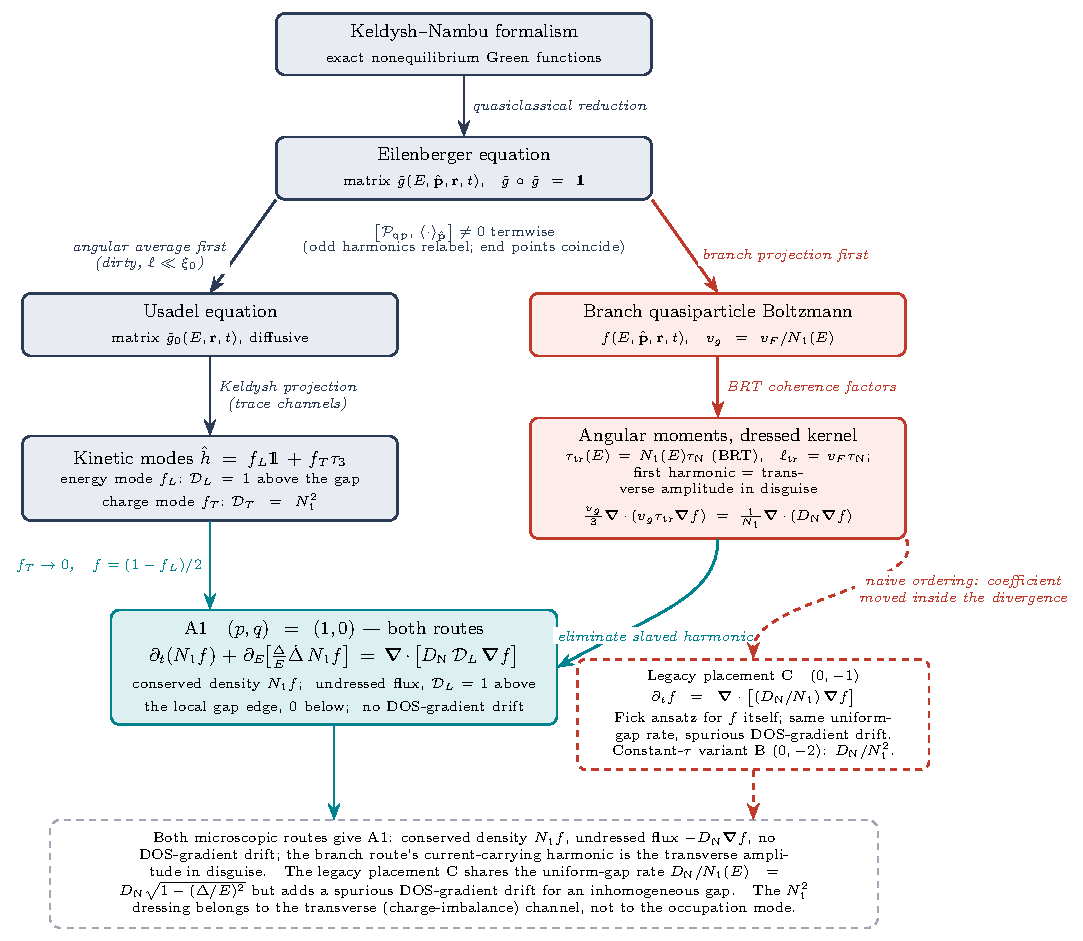
\includegraphics[width=0.84\textwidth]{figures/routes_roadmap}
  \caption{Reduction routes from the quasiclassical matrix theory to the
  candidate diffusion operators of \cref{tab:operator_taxonomy}. The two
  branches perform the same pair of operations---Nambu/branch projection
  and angular averaging---in opposite order, and the operations do not
  commute termwise (\cref{sec:projection_vs_averaging}): the
  relabelling shuffles odd angular harmonics between the longitudinal and
  transverse sectors. Their scalar end points nevertheless coincide: the
  matrix (dirty) route and the branch route with the
  Bardeen--Rickayzen--Tewordt-dressed kernel both fix the longitudinal
  operator A1, \((p,q)=(1,0)\): conserved spectral density \(\DOS f\),
  undressed flux (\(\mathcal{D}_L=1\) above the local gap edge, \(0\)
  below), no DOS-gradient drift, with the squared-DOS dressing
  \(\mathcal{D}_T=\DOS^2\) residing in the transverse (charge-imbalance)
  channel. The legacy placement C, \((0,-1)\), shares the uniform-gap
  rate \(\DN/\DOS(E)\) but is a Fick ansatz for the occupation itself,
  not the end point of either route; its DOS-gradient drift is the
  artifact the benchmarks quantify.}
  \label{fig:routes_roadmap}
\end{figure*}

\begingroup
\squeezetable
\begin{table*}[!tbp]
\caption{\label{tab:operator_taxonomy}Candidate diffusion operators collected
for the manuscript. Here \(\DOS=\DOS(E,\Delta)\). Both microscopic routes
select A1: the dirty-limit Keldysh--Usadel projection (\(q=0\): the matrix
flux is undressed above the local gap edge and blocked below it, \(p=1\)
from quasiparticle-number continuity, with the time-dependent
spectral-flow term produced directly by the fixed-\(E\) projection,
\cref{sec:tdep_spectral_flow}), and equally the branch-projected moment
reduction with the BRT-dressed kernel
[\cref{eq:sc_scalar_diffusion,eq:sc_tau_closure}]. The \((0,\cdot)\)
rows B and C are \emph{legacy placements}---Fick ans\"atze for the
occupation \(f\) itself, with the whole coefficient inside the
divergence; they are retained as labeled diagnostics of the naive
operator ordering, not as route end points. The \((1,2)\) row attaches
the \emph{transverse} (charge-imbalance) flux dressing
\(\mathcal{D}_T=\DOS^2\) of \cref{eq:DL_DT_BCS_bulk} to the occupation
mode; it is not selected by the Keldysh projection and is kept
only as a labeled diagnostic. A2 is a nonstandard symmetric test operator.}
\begin{ruledtabular}
\begin{tabular}{p{0.16\textwidth}p{0.09\textwidth}p{0.22\textwidth}p{0.28\textwidth}p{0.11\textwidth}}
Name & Label & Route & Operator & Uniform-\(\Delta\) rate \\
\hline
Usadel, QP-number closure & A1: \((1,0)\) &
Matrix angular average, scalar projection, conserved density \(\DOS f\),
undressed flux (\(\mathcal{D}_L\)) &
\(\DN\DOS^{-1}\bnabla\cdot(\mathcal{D}_L\bnabla f)\) &
\(\DN\mathcal{D}_L/\DOS\) \\
Transverse-flux dressing (charge channel) & A1\('\): \((1,2)\) &
Diagnostic: attaches the transverse coefficient
\(\mathcal{D}_T=\DOS^2\) to the occupation mode &
\(\DN\DOS^{-1}\bnabla\cdot(\DOS^2\bnabla f)\) &
\(\DN\DOS\) \\
Usadel-flux symmetric test & A2: \((2,2)\) &
Transverse-dressed flux, nonstandard conserved density \(\DOS^2 f\) &
\(\DN\DOS^{-2}\bnabla\cdot(\DOS^2\bnabla f)\) &
\(\DN\) \\
Legacy placement, constant \(\tau\) & B: \((0,-2)\) &
Naive ordering: constant-\(\tau\) coefficient inside the divergence
(Fick ansatz for \(f\)); the ordered branch reduction instead gives
\((1,-1)\), the continuity-skeleton member with \(\DE=\DN/\DOS^{2}\),
not benchmarked separately &
\(\bnabla\cdot[(\DN/\DOS^2)\bnabla f]\) &
\(\DN/\DOS^2\) \\
Legacy placement, BRT / constant \(\ell\) & C: \((0,-1)\) &
Naive ordering: BRT coefficient inside the divergence (Fick ansatz for
\(f\)); the ordered branch reduction gives A1 &
\(\bnabla\cdot[(\DN/\DOS)\bnabla f]\) &
\(\DN/\DOS\) \\
Continuity skeleton & \(p=1\) &
Conserved density \(\DOS f\), mobility unspecified &
\(\DOS^{-1}\bnabla\cdot[\DOS\DE\bnabla f]\) &
\(\DE\) if \(\DOS\) uniform \\
\end{tabular}
\end{ruledtabular}
\end{table*}
\endgroup

The table separates microscopic limits from diagnostic closures.
A1 is the end point of \emph{both} microscopic routes: the dirty-limit
Keldysh--Usadel scalar projection, and equally the branch-projected
moment reduction once its operator ordering
[\cref{eq:sc_scalar_diffusion}] and the BRT-dressed kernel
[\cref{eq:sc_tau_closure}] are kept---conserved density \(\DOS f\), undressed flux, uniform-gap rate
\(\DN/\DOS(E)\), with the time-dependent spectral-flow term produced
directly by the fixed-\(E\) projection (\cref{sec:tdep_spectral_flow}).
C is the legacy placement of the same BRT coefficient inside the
divergence---a Fick ansatz for the occupation \(f\), widely used in
device modeling (e.g., it is the energy-resolved starting point,
Appendix~A, of the gap-engineered-trap analysis of
Ref.~\onlinecite{riwar2019}); it shares the uniform-gap rate of A1, which is why the
misplacement goes unnoticed until the gap is inhomogeneous, where it
adds the \(q=-1\) DOS-gradient drift of \cref{eq:Lpq_expanded}. B is the
same placement with the undressed constant-\(\tau\) coefficient, which
additionally misses the coherence-factor cancellation. The \((1,2)\)
entry is retained only to label the transverse-channel flux
dressing---the Keldysh projection does not attach it to the occupation
mode (\cref{eq:DL_DT_BCS_bulk})---and A2 further replaces the time
weight by the nonstandard \(\DOS^2 f\); both are diagnostics, not Usadel
derivations. If the continuity skeleton's mobility is later chosen as
\(\DE=\DN\DOS^r\), its \((p,q)\) label is \((1,r+1)\); in particular,
\(r=-1\) recovers A1, now reached from three directions: the
Usadel--continuity closure, the dirty matrix projection, and the ordered
branch reduction.

\section{Consistency checks and benchmark tests}
\label{sec:program}

The comparison above reduces the problem to a small set of explicit
checks and benchmarks. Two pieces are fixed by standard theory: the
dirty-limit projection selects A1 (\cref{sec:usadel_route}), and the BRT
coherence-factor cancellation fixes the branch-route kernel, whose
ordered reduction [\cref{eq:sc_scalar_diffusion,eq:sc_tau_closure}] lands on the same A1.
This section states the regime boundaries,
interface reductions, and crossover tests that distinguish the candidate
operators, and then benchmarks the resulting operators numerically.

\subsection{Projection versus angular averaging}
\label{sec:projection_vs_averaging}

The Usadel route averages over momentum directions before extracting a
scalar quasiparticle occupation. The scalar Boltzmann route extracts the
branch occupation first and averages later. The two routes therefore apply
the same pair of operations in opposite order, and termwise the operations
do not commute:
\begin{equation}
  \left[
    \mathcal{P}_{\qp},
    \avg{\cdot}_{\hat{\bp}}
  \right]\check{g}
  \neq 0.
  \label{eq:projection_average_commutator}
\end{equation}
The non-commutation is real but is exhausted by a relabelling: the
branch-to-trajectory map acts on odd angular harmonics
[\cref{eq:intro_parity_dictionary}], so the branch
route's current-carrying first harmonic is the anisotropic
\emph{transverse} amplitude of the two-mode description in
disguise---while the isotropic charge-imbalance mode is the component
that vanishes in the charge-balanced sector. Eliminating that slaved
harmonic reproduces the same longitudinal operator as the matrix route,
as the hidden-harmonic map \cref{eq:sc_hidden_harmonic} and the
closed operator \cref{eq:sc_LD_closed} show explicitly: the scalar end points coincide on A1
(\cref{fig:routes_roadmap}). The commutator therefore marks a boundary
between representations, not between diffusion laws; genuinely different
kinetics appears only outside the shared assumptions---ballistic
transport with mean free paths comparable to device scales,
proximity-modified spectra, charge imbalance, and the extensions bounded
in the SM.

\subsection{Conserved density and boundary conditions}

Spatial diffusion in devices is also a boundary-value problem. Matrix Usadel
theory has current-conserving boundary conditions at interfaces, including the
Kupriyanov--Lukichev condition for low-transparency diffusive interfaces
\cite{kupriyanov1988}. A scalar diffusion model must specify the corresponding
conserved scalar current:
\begin{equation}
  \mathbf{j}_E
  =
  -\mathcal{W}(E,\br)\,\mathcal{D}(E,\br)\,
  \bnabla_{\br}f,
  \label{eq:generic_energy_current}
\end{equation}
including the weight \(\mathcal{W}\), mobility \(\mathcal{D}\), and matching
conditions across spatially varying \(\Delta(\br)\), material interfaces, or
trapping regions.

The scalar boundary condition should be obtained by projecting the
Kupriyanov--Lukichev matrix-current relation onto the same longitudinal
occupation used in the bulk equation. In a scalar model this projection must
identify three objects: the interface weight \(\mathcal{W}\), the mobility
\(\mathcal{D}\), and the jump condition for either \(f\), \(\DOS f\), or any
nonstandard weighted scalar retained as a benchmark. Without this matching step,
two bulk operators that look reasonable can still impose incompatible interface
currents.

\paragraph{Result of the projection.} Carrying this out for a low-transparency
(Kupriyanov--Lukichev) tunnel interface between BCS electrodes \(1,2\) --- taking
the plain-trace longitudinal component of the matrix interface current
\((2R_bA)^{-1}[\check{g}_1,\check{g}_2]^{K}\) --- gives
\begin{equation}
  j_L=G_N\!\left[\DOS^{(1)}\DOS^{(2)}-N_2^{(1)}N_2^{(2)}\right]\!
  \bigl(\fL^{(1)}-\fL^{(2)}\bigr),
  \qquad G_N=(R_bA)^{-1},
  \label{eq:scalar_BC_energy}
\end{equation}
the coherence-factor (Maki--Griffin heat-current) weight~\cite{maki1965}. The three objects of
\cref{eq:generic_energy_current} are therefore the interface weight
\(\mathcal{W}=\DOS^{(1)}\DOS^{(2)}-N_2^{(1)}N_2^{(2)}\), the
mobility \(\mathcal{D}=G_N\), and the jump variable: the quantity continuous
across the interface is the \emph{current}, not \(f\) or \(\DOS f\); the bare
occupation \(f\) jumps, and matching the interface current to the undressed
bulk flux \(-\DN\,\mathcal{D}_L\bnabla\fL\) on each side yields a Robin
condition.
The charge (transverse) channel decouples, carrying the density-of-states
product \(\DOS^{(1)}\DOS^{(2)}\) familiar from SIS quasiparticle tunneling;
both weights reduce to the superconductor density of states at a
normal-metal contact. The gap-edge singularity structure separates cleanly
by channel: at matched gaps the energy weight is regular
(\(\DOS^2-N_2^2=1\)), while the charge weight \(\DOS^{(1)}\DOS^{(2)}\)
carries the matched-gap edge singularity familiar from the SIS
current--voltage characteristic. The detailed projection is given in SM~\cref{SM-app:derivation}.

\subsection{Self-consistent gap feedback}
\label{sec:self_consistent_feedback}

The first three benchmarks below treat \(\Delta(\br)\) as prescribed. In a device the
gap is not free: the occupation enters the BCS gap equation, and any
population suppresses the local order parameter
\cite{owen1972,parker1975}. Dividing the local weak-coupling gap
equation [cf.~\cref{eq:intro_three_gap}],
\(1=\lambda\int_0^{\omega_c}\dd\xi\,[1-2f(E)]/E\), by its
equilibrium counterpart cancels the cutoff (\(\omega_c\gg\Delta\)) and
gives the closed local form
\begin{equation}
  \Delta(\br)
  =
  \Delta_0\,
  \exp\!\left[
    -2\int_{\Delta}^{\infty}\frac{\dd E}{E}\,\DOS(E,\br)\,f(E,\br)
  \right],
  \label{eq:gap_feedback_closure}
\end{equation}
with \(\DOS\) evaluated at the self-consistent local gap. No
linearization is involved: a thermal occupation in
\cref{eq:gap_feedback_closure} reproduces the equilibrium \(\Delta(T)\),
and a nonequilibrium population suppresses the gap beyond it. For a
small exponent the familiar linear response
\(\delta\Delta/\Delta_0=-2\int(\dd E/E)\,\DOS f\) follows, reducing for
a population concentrated near the gap edge to \(-x_{\qp}(\br)\), where
\(x_{\qp}=n_{\qp}/(2N_0\Delta_0)\) and
\(n_{\qp}=4N_0\int\DOS f\,\dd E\), \(N_0\) being the single-spin
normal-state density of states at the Fermi level. The amplitude is small in devices
(\(x_{\qp}\sim10^{-9}\)--\(10^{-5}\) in qubits, larger under drive), but
the drift \emph{response} of the transport operators to it is governed
by the density-of-states gradient, which is singular at the gap
edge: at fixed energy,
\begin{equation}
  \bnabla\ln\DOS(E,\br)
  =
  \frac{\Delta\,\bnabla\Delta(\br)}{E^2-\Delta^2},
  \label{eq:dos_gradient_response}
\end{equation}
which diverges as \(E\to\Delta\)---precisely where thermal and
nonequilibrium populations concentrate. Every \(q\neq0\) member of
\cref{eq:Lpq_expanded} converts this into the drift
\(v=\DN\,q\,\DOS^{\,q-p-1}\partial_x\DOS\), with the sign of \(q\)---divergent
at the edge for \(q-p>-2\) and finite precisely at the marginal exponent
\(q-p=-2\) of the legacy placement B; the
dirty-limit operator A1 (\(q=0\)) has no drift response at any amplitude.

Two statements keep the feedback from threatening the A1 reduction
itself. First, the combined background \(\Delta(\br,t)\) that
self-consistency generically produces adds no new terms to the
longitudinal projection: the fixed-\(E\) trace yields the spectral flow
with local coefficients, the spatial current remains undressed with no
\(\bnabla\Delta\) source, the drive does not mix the scalar channels, and
the first Moyal correction to \(g_0^K\) is sourced only by \(\fT\), so
the leading candidate \(\hbar\,\dot\Delta\,\partial_x\Delta\) cross term
traces to zero in the energy mode (verified symbolically alongside the
identities of \cref{sec:tdep_spectral_flow}). Self-consistency changes
the \emph{background} A1 runs on, not the operator. Second, the feedback
makes the inhomogeneous-gap regime self-generating: a localized
population digs its own gap well, so the structure that separates the
candidate operators is engaged without any externally imposed profile.
The fourth benchmark below realizes exactly this configuration.

\subsection{Benchmark problems}

Four benchmark problems separate the models cleanly:
\begin{enumerate}
  \item a uniform-gap Gaussian packet, where the microscopic operator A1
  \((p,q)=(1,0)\) and the legacy constant-\(\ell\) placement C share the
  near-gap-suppressed rate \(\DN/\DOS(E)\), while the diagnostic closures
  separate from them: the \((1,2)\) operator gives a rate
  \(\DN\DOS(E)\) that diverges at the gap edge, A2 \((p,q)=(2,2)\) gives
  the energy-independent rate \(\DN\), and the constant-\(\tau\) placement
  suppresses the rate more strongly as \(\DN/\DOS^2\);
  \item a spatially varying gap with no collisions, where A1
  carries \emph{no} DOS-gradient drift (the inhomogeneity enters only
  through \(\mathcal{D}_L\) and the outside spectral factor), the legacy
  placement C carries the spurious drift of its \(q=-1\) flux, and the \(q=2\)
  diagnostics drift with the opposite sign and, asymptotically
  (\(E\gg\Delta\)), twice the magnitude;
  \item an interface or trap geometry---the configuration of engineered
  quasiparticle traps \cite{riwar2016,hosseinkhani2018,riwar2019}---where conservation of the integrated
  quasiparticle number can be tested against boundary conditions, and where
  A1 (which conserves \(\DOS f\) by construction) and A2 (which conserves
  \(\DOS^2 f\)) can be distinguished by the equilibrium they relax to;
  \item a self-consistent feedback problem, in which a localized
  quasiparticle population digs its own gap well through the gap
  closure \cref{eq:gap_feedback_closure}, and a weak probe packet on the
  well's flank reads out each operator's drift response to the
  self-generated DOS gradient.
\end{enumerate}
The first benchmark tests the rate spectrum: the agreeing pair
A1/constant-\(\elltr\), the diagnostic \((1,2)\) and A2 operators, and
constant-\(\tau\) make different predictions even before boundaries or gap
gradients are introduced. The second
tests the DOS-gradient drift dressing, which \emph{distinguishes} the
microscopic operator from the legacy placement that shares its
uniform-gap rate. The third tests whether the scalar
current is the correct reduction of the matrix spectral current and which scalar
density it conserves. The fourth closes the loop of
\cref{sec:self_consistent_feedback}: it asks whether quasiparticles
respond to the gap landscape they themselves create, and with which sign.

\Cref{fig:bench_uniform,fig:bench_drift,fig:bench_interface} realize the
first three tests numerically, treating every operator with the same
one-dimensional Crank--Nicolson discretization---time evolution for the
drift and interface tests, a single exact inversion of the amplification
factor for the uniform-gap rates (aluminum-strip
parameters, \(\DN=6~\mu\mathrm{m}^2/\mathrm{ns}\),
\(L=100~\mu\mathrm{m}\), reflective ends; the \((1,2)\) diagnostic
A1\('\) is labeled A1P in the legends). The measured points sit on the analytic
spectra in all three problems: the uniform-gap rates trace
\(\DOS^{\,q-p}\), with A1 and C coincident on \(\DN/\DOS\)
(\cref{fig:bench_uniform}); the ramp drift velocities---measured on the center of mass of each
operator's conserved density \(\DOS^{p}f\)---trace
\(\DN\,q\,\DOS^{\,q-p-1}\partial_x\DOS\), with A1 driftless and the
\(q=2\) diagnostics moving opposite to the legacy placements
(\cref{fig:bench_drift}); and the interface problem separates the
conserved densities, A1 and A2 relaxing to distinct closed-box equilibria
while both carry a continuous current through the Kupriyanov--Lukichev
face (\cref{fig:bench_interface}).

\begin{figure}[t]
  \centering
  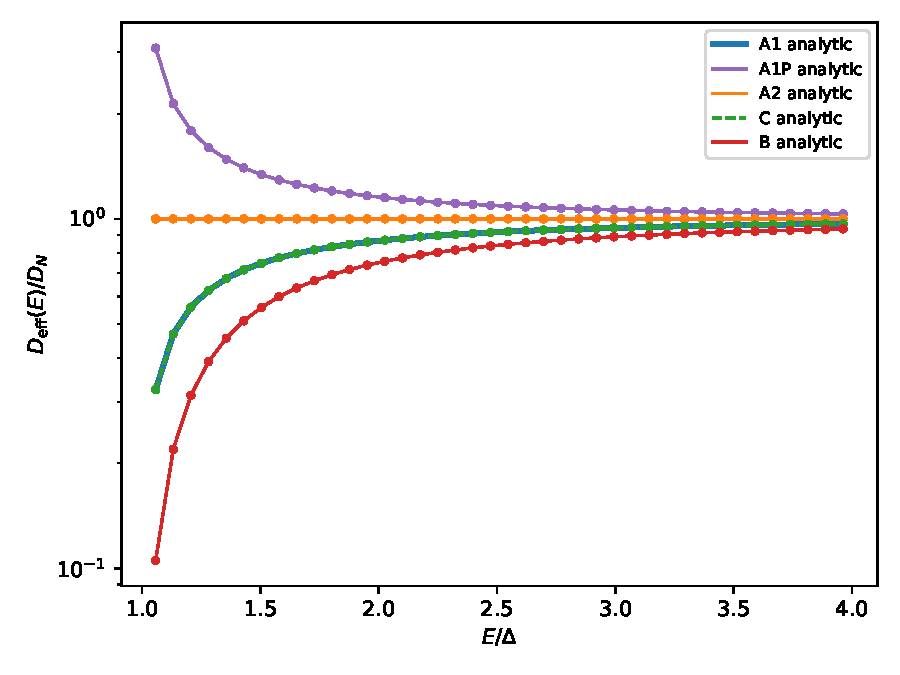
\includegraphics[width=0.62\textwidth]{figures/uniform_gap_packet}
  \caption{Uniform-gap benchmark: energy-resolved effective diffusivity
  \(D_{\mathrm{eff}}(E)/\DN\) for the five scalar operators. Lines are
  the analytic spectra \(\DOS^{\,q-p}\); markers are measured from a
  single exact inversion of the Crank--Nicolson amplification of the
  fundamental reflective spatial mode. The microscopic operator
  A1, \((p,q)=(1,0)\) (wide line), and the legacy constant-\(\elltr\)
  placement C, \((0,-1)\) (dashed), coincide on the near-gap-suppressed
  rate \(\DN/\DOS(E)\); the transverse-dressed \((1,2)\) diagnostic
  rises as \(\DOS\), A2 \((2,2)\) is energy independent, and the
  constant-\(\tau\) placement B \((0,-2)\) is suppressed as
  \(\DOS^{-2}\). The integrated quasiparticle number is conserved to
  round-off (\(\lesssim10^{-15}\) relative) by every operator.}
  \label{fig:bench_uniform}
\end{figure}

\begin{figure}[t]
  \centering
  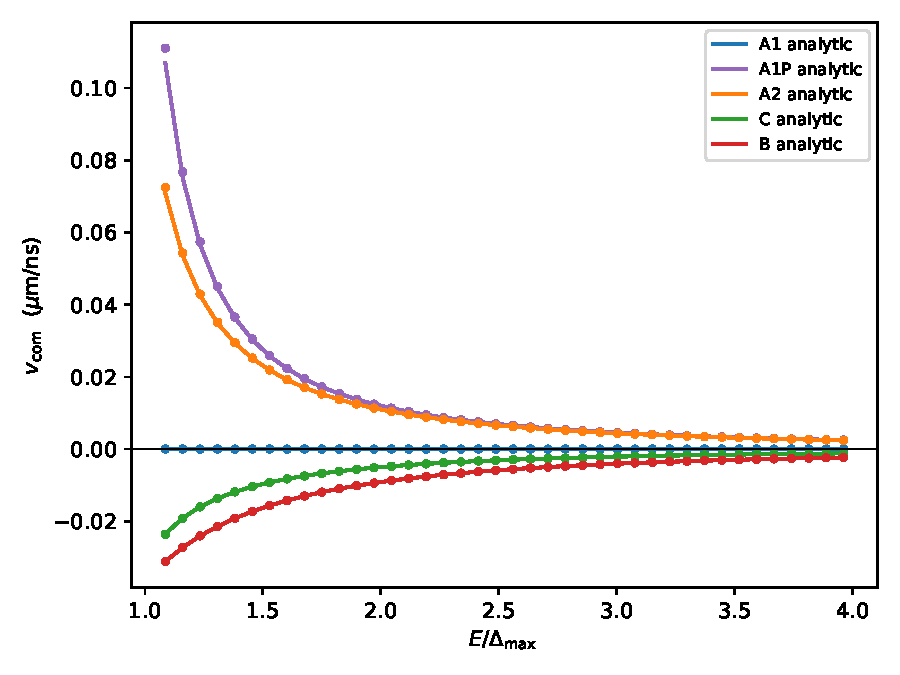
\includegraphics[width=0.62\textwidth]{figures/gap_gradient_drift}
  \caption{Gap-gradient benchmark: center-of-mass drift velocity,
  energy by energy, of a Gaussian packet (\(\sigma=8~\mu\mathrm{m}\)) on
  a static linear ramp \(\Delta(x)\) rising from \(\Delta_0\) to
  \(1.6\,\Delta_0\) across the strip, with no collisions. Lines are the
  analytic drift \(v=\DN\,q\,\DOS^{\,q-p-1}\,\partial_x\DOS\); markers
  are measured. The tracked moment is the center of mass of each
  operator's conserved density \(\DOS^{p}f\), which isolates the drift
  content of the flux; the first moment of \(f\) itself would
  additionally respond to the spatially varying rate prefactor
  \(\DOS^{\,q-p}(x)\). A1 (\(q=0\)) shows no DOS-gradient drift; the \(q=2\)
  diagnostics drift up the gap gradient; the legacy placements C
  (\(q=-1\)) and B (\(q=-2\)) drift down, with magnitudes set
  asymptotically by \(q\).}
  \label{fig:bench_drift}
\end{figure}

\begin{figure}[t]
  \centering
  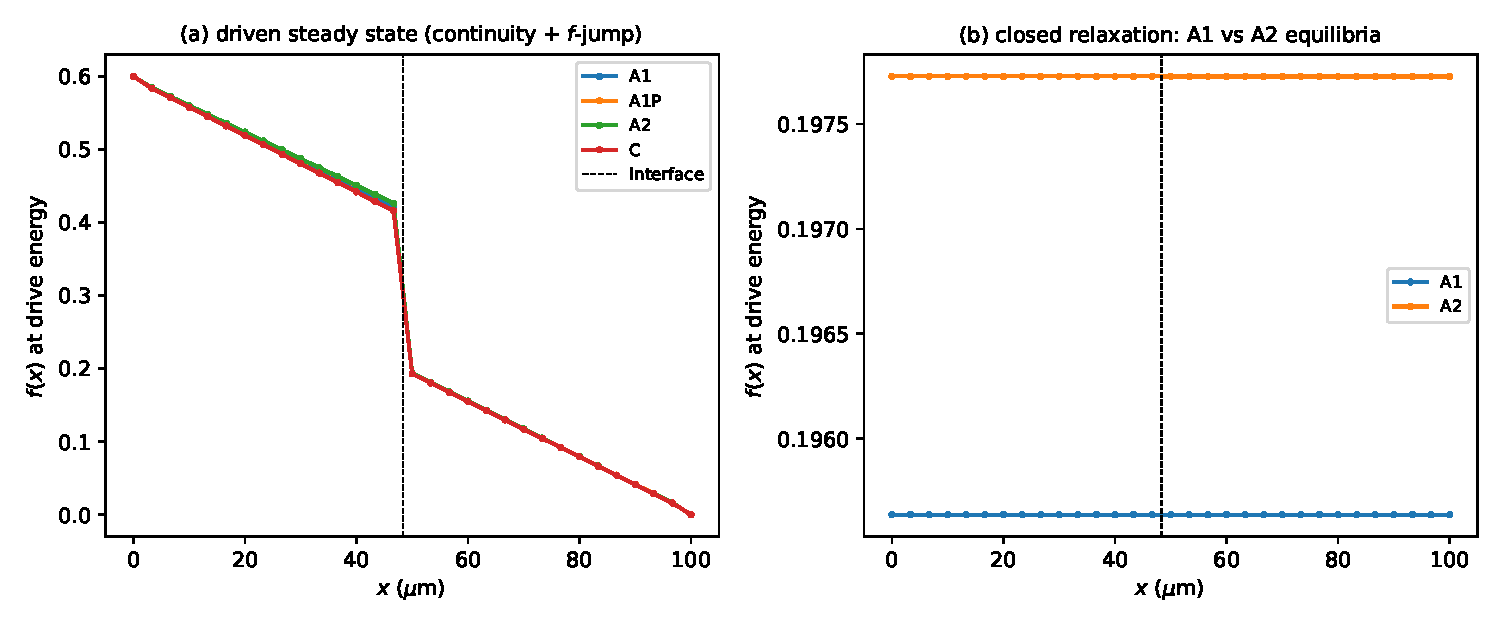
\includegraphics[width=\textwidth]{figures/interface_trap}
  \caption{Interface benchmark: a two-gap strip (\(1.6\,\Delta_0\) for
  \(x<50~\mu\mathrm{m}\), \(\Delta_0\) beyond) joined by a
  Kupriyanov--Lukichev face carrying the coherence-factor weight of
  \cref{eq:scalar_BC_energy} (\(G_N=0.1\)), shown at a fixed energy
  above both gap edges. (a)~Driven steady state with a fixed-\(f\)
  source at the left edge: every operator carries equal currents on the
  faces left of, at, and right of the interface (continuity to solver
  tolerance), with an operator-dependent \(f\)-discontinuity at the
  face. (b)~Closed-box relaxation from a common initial condition: A1
  and A2 relax to \emph{distinct} flat equilibria---they conserve
  \(\DOS f\) and \(\DOS^{2}f\), respectively---differing by
  \(\sim2\times10^{-3}\) at the drive energy.}
  \label{fig:bench_interface}
\end{figure}

\Cref{fig:bench_feedback} realizes the fourth test with the same
discretization (well depth \(\delta\Delta/\Delta_0=0.05\) dug by a
maintained near-edge population of width \(10~\mu\mathrm{m}\); probe read
out at \(E=1.08\,\Delta_0\)). In the quasi-static well the probe's
conserved-density center of mass reproduces the analytic drift spectrum
evaluated on the self-generated profile: the legacy placements
fall \emph{into} the well their own population dug (C and B within a few
percent of the prediction), the \(q=2\) diagnostics are expelled from
it, and A1 does not move---zero to round-off, since its undressed face
flux telescopes across the well. With fully dynamic feedback (the gap
tracking the population every step) the same signature survives; the
bookkeeping drift from the neglected energy-space spectral-flow
advection is measured rather than hidden, at the percent level for the
\(p\geq1\) operators over the \(20\)-ns run and zero for \(p=0\).
Self-focusing into self-generated gap suppression is therefore a
structural artifact of the \(q<0\) legacy placements; the microscopic
operator---by either route---predicts no self-focusing.

\begin{figure}[t]
  \centering
  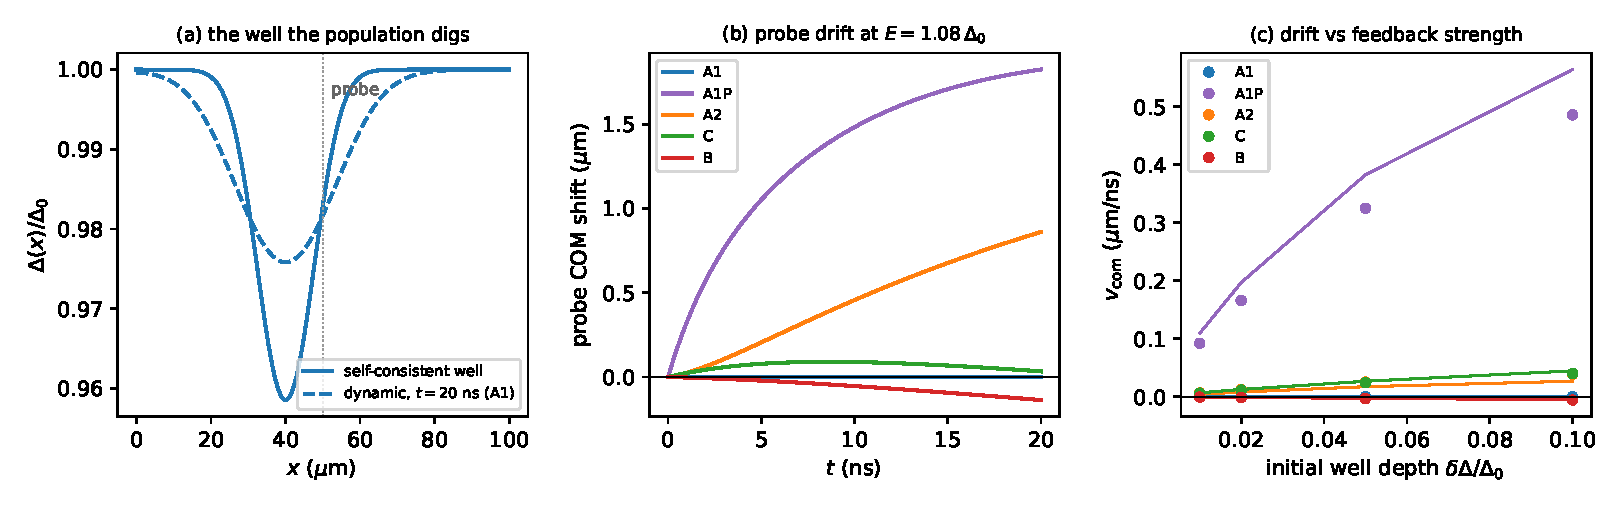
\includegraphics[width=\textwidth]{figures/self_consistent_feedback}
  \caption{Self-consistent feedback benchmark. (a)~The gap well dug by a
  localized quasiparticle population through the gap closure
  \cref{eq:gap_feedback_closure} (solid; target depth
  \(\delta\Delta/\Delta_0=0.05\)), and the same well after \(20\)~ns of
  fully dynamic feedback under A1 (dashed); the dotted line marks the
  probe packet on the flank. (b)~Probe center-of-mass drift at
  \(E=1.08\,\Delta_0\) in the quasi-static well: the legacy placements C
  and B fall toward the well, the \(q=2\) diagnostics A1\('\) (legend:
  A1P) and A2 are
  expelled, and the microscopic A1 stays exactly put. (c)~Measured
  (markers) versus analytic (lines) drift velocity at the probe versus
  well depth: the response scales with the feedback strength with the
  sign of \(q\), and A1's vanishing drift is parameter-free.}
  \label{fig:bench_feedback}
\end{figure}

\section{Conclusion}

Within its assumptions---local BCS spectra, nonmagnetic Born disorder,
negligible charge imbalance---the bulk energy-resolved scalar diffusion
operator is not a free modeling choice: it has a single
microscopically selected form, and both reduction routes deliver it.
The matrix Usadel route gives a
first-principles dirty-limit longitudinal spectral current that is
\emph{undressed} above the local gap edge and blocked below it
(\(\mathcal{D}_L=1\) and \(0\), respectively), and its scalar projection
fixes the quasiparticle-number
continuity equation A1, \((p,q)=(1,0)\): the conserved
energy-resolved scalar is \(\DOS f\), and the uniform-gap rate is
\(\DN/\DOS(E)\). The \(\DOS^2\) flux dressing belongs to the transverse
(charge-imbalance) channel, \(\mathcal{D}_T=\DOS^2\). On a uniform
time-dependent background the spectral-flow term
\((\Delta/E)\dot\Delta\,\partial_E f\) is produced directly by the
fixed-\(E\) scalar projection of the matrix equation; lifting the conserved
scalar to the moving quasiparticle energy shell reproduces it and supplies
its kinematic interpretation
(\cref{sec:tdep_spectral_flow}). New content
beyond A1 requires leaving the present assumptions---a supercurrent,
proximity-modified spectra, or nonadiabatic dynamics;
SM~\cref{SM-app:supercurrent,SM-app:proximity,SM-app:nonadiabatic}
derive, estimate, or bound the leading correction in each case. The symmetric A2
operator, \((p,q)=(2,2)\), attaches the transverse flux dressing to the
occupation mode with a \(\DOS^2 f\) time weight; it is a diagnostic
test operator, not an independent microscopic consequence of Keldysh--Usadel.

In the scalar quasiparticle Boltzmann route, the
Bardeen--Rickayzen--Tewordt coherence-factor cancellation selects a
constant transport mean free path, \(\DOS D_{\mathrm B}=\DN\), and the
moment reduction lands on the same operator A1 as the dirty-limit
projection: the same conserved density, the same undressed flux, no
DOS-gradient drift. The legacy device-physics coefficient
\(\DN/\DOS(E)\) is therefore microscopically supported in both routes,
but its common placement inside the divergence,
\(\bnabla\cdot[(\DN/\DOS)\bnabla f]\), is not: it treats the occupation
as the conserved density and acquires a spurious DOS-gradient drift for
an inhomogeneous gap. The remaining theoretical
task is to map the regimes and crossovers in which the A1 reduction
gives way to ballistic kinetics, proximity-modified spectra, or
interface- and trap-dominated transport.

For device modeling, A1 does not by itself close an equation for the
spatially resolved \emph{total} quasiparticle density
\(n_{\qp}(\br,t)=4N_0\int_\Delta^\infty\DOS(E)\,f(E,\br,t)\,\dd E\), with \(N_0\)
the single-spin normal-state density of states at the Fermi level (the
factor \(4\) counting spin and the two branches \(\pm\xi\)); an
additional closure is required.
Integrating the energy-resolved A1 equation over \(E\) under a fixed
spectral shape or local-equilibrium closure, the effective macroscopic
diffusion constant is an energy average of \(\DN/\DOS(E)\) weighted by the
population: near-gap quasiparticles, which dominate the thermal population
at \(T\ll\Delta\) where \(\DOS\) is largest, carry a \emph{suppressed}
diffusive weight in both microscopic routes---a statement about the bulk
operator away from the gap-edge boundary layer, where the moment
reduction itself degrades (\cref{sec:sc_transport_closures}). What the operator placement
changes in spatially
resolved Rothwarf--Taylor models~\cite{rothwarf1967} is the
inhomogeneous-gap structure of the flux---sub-gap blocking and the absence
of a DOS-gradient drift in the microscopic operator. Because the local gap is
itself suppressed by the quasiparticle population
\cite{owen1972,parker1975}, a spatially resolved simulation generates gap
inhomogeneity dynamically wherever the density is nonuniform: the
inhomogeneous-gap structure of the operator is engaged---at some
amplitude---in any self-consistent device model, not only in deliberately
gap-engineered geometries. The feedback benchmark of
\cref{sec:self_consistent_feedback} makes the distinction concrete: under
the legacy \(q=-1\) placement a packet drifts into the gap well its own
population digs, while the microscopic operator predicts no such
self-focusing.

Finally, the local-BCS scalar operators above are not expected to hold
where the spectral
functions vary on the scale of the coherence length, or where a single conserved
scalar is ill-defined: vortex cores, strongly inhomogeneous or
proximity-suppressed gaps, and regimes with significant charge imbalance or
branch coherence. In the dirty quasiclassical regime this requires the
two-component matrix Keldysh--Usadel equations (and the Eilenberger or BdG level
for clean systems); for weakly proximity-modified spectra the
leading-order scalar corrections are organized in
SM~\cref{SM-app:proximity}.


\begin{acknowledgments}
This work was supported by the NASA Astrophysics Research and Analysis
(APRA) program under solicitation NNH21ZDA001N (``Modeling and Testing
KIDs for Astrophysics,'' PI: P.~Timbie).
\end{acknowledgments}

\paragraph*{Data and code availability.}
The computer-algebra scripts that verify every identity cited in the text
and in the Supplemental Material are available at
\url{https://github.com/Soren-O/qp-diffusion-verification}. The benchmark
figures were generated with the \texttt{diffusion\_operators} validation
module of the open-source \texttt{qpsim} simulation package,
\url{https://github.com/Soren-O/Quasiparticle-Physics-Simulation}.

\appendix

\section{Explicit change of variables \texorpdfstring{\(\bk\to(E,\hat{\bk})\)}{k -> (E,k)}}
\label{app:change_of_variables}

This appendix records, component by component, the change of variables
behind the energy--angle form of \cref{eq:intro_boltzmann_clean}; the
substitution is elementary but rarely written out.
Since \(E_{\bk}(\br,t)\) depends on position and time through
\(\Delta(\br,t)\), derivatives taken at fixed \(\bk\) and at fixed
\(E\) differ. We make use of the identity: for a function written as
\(g(z,y)=g(x(z,y),y)\),
\begin{equation}
\left(\frac{\partial g}{\partial y}\right)_z
=
\left(\frac{\partial g}{\partial x}\right)_y
\left(\frac{\partial x}{\partial y}\right)_z
+
\left(\frac{\partial g}{\partial y}\right)_x .
\end{equation}
And for a gradient, resolved into radial and angular parts,
\begin{equation}
\bnabla_{\br} f(r,\hat{\br})
=
\hat{\br}\,\frac{\partial f}{\partial r}
+
\frac{1}{r}\,\bnabla_{\hat{\br}} f ,
\end{equation}
with \(\bnabla_{\hat{\br}}\) the gradient on the direction sphere.
Applied individually to the three derivatives of \(f_{\bk}\) that
appear in \cref{eq:intro_canonical_boltzmann}, this gives
\begin{align}
  \Bigl(\frac{\partial f}{\partial t}\Bigr)_{\!\bk}
  &=
  \Bigl(\frac{\partial f}{\partial t}\Bigr)_{\!E}
  +
  \Bigl(\frac{\partial E_{\bk}}{\partial t}\Bigr)_{\!\bk}
  \frac{\partial f}{\partial E},
  \label{eq:intro_chain_t}
  \\
  \bigl(\bnabla_{\br}f\bigr)_{\bk}
  &=
  \bigl(\bnabla_{\br}f\bigr)_{E}
  +
  \bigl(\bnabla_{\br}E_{\bk}\bigr)_{\bk}\,
  \frac{\partial f}{\partial E},
  \label{eq:intro_chain_r}
  \\
  \frac{\partial f}{\partial\bk}
  &=
  \hat{\bk}\,\frac{\partial f}{\partial k}
  +
  \frac{1}{k}\,\bnabla_{\hat{\bk}} f ,
  \label{eq:intro_p_basic}
\end{align}
the first two using the chain-rule identity and the last the gradient
identity with \(\br\to\bk\). The fixed-\(\bk\) time and space
derivatives, nonzero only because \(\Delta(\br,t)\) moves, are
\begin{equation}
  \Bigl(\frac{\partial E_{\bk}}{\partial t}\Bigr)_{\!\bk}
  =
  \frac{\Delta}{E}\,\dot{\Delta},
  \qquad
  \mathbf{F}_{\Delta}
  \equiv
  -\bigl(\bnabla_{\br}E_{\bk}\bigr)_{\bk}
  =
  -\frac{\Delta}{E}\,\bnabla_{\br}\Delta .
  \label{eq:intro_E_derivatives}
\end{equation}
For the momentum line, the radial derivative runs through the
dispersion by the chain rule \(\partial f/\partial k=(\partial
E_{\bk}/\partial k)\,\partial f/\partial E\); since
\(\hbar^{-1}\partial E_{\bk}/\partial\bk=\bv_{\mathrm{g}}\), the radial part is
\(\hat{\bk}\,\partial f/\partial k=\hbar\,\bv_{\mathrm{g}}\,\partial f/\partial E\).
The angular part is transverse: \(\hat{\bk}=\bk/k\) has Jacobian
\(\partial\hat{\bk}/\partial\bk=k^{-1}(\openone-\hat{\bk}\hat{\bk})\), so
the surface gradient enters projected onto the tangent plane as
\((\openone-\hat{\bk}\hat{\bk})\cdot\bnabla_{\hat{\bk}}f\), and a
contraction with any momentum-space vector keeps only its component
along the Fermi sphere. \Cref{eq:intro_p_basic} thus becomes
\begin{equation}
  \frac{\partial f}{\partial\bk}
  =
  \hbar\,\bv_{\mathrm{g}}\,\frac{\partial f}{\partial E}
  +
  \frac{1}{k}\,
  \bigl(\openone-\hat{\bk}\hat{\bk}\bigr)
  \cdot
  \bnabla_{\hat{\bk}} f .
  \label{eq:intro_p_derivative}
\end{equation}
Substituting these into \cref{eq:intro_canonical_boltzmann}---and
setting \(k\to k_{\mathrm F}\) in the angular term, a relative error
\(O(|\xi_{\bk}|/E_{\mathrm F})\) (i.e.\ \(O(\Delta/E_{\mathrm F})\) for
near-gap quasiparticles, at most \(O(\omega_D/E_{\mathrm F})\) across the
pairing shell) that is quasiclassically negligible---gives the
Boltzmann-like equation with ballistic (clean-limit) streaming, now in
the \((E,\hat{\bk})\) variables,
\begin{equation}
\begin{aligned}
\Bigl(\frac{\partial f}{\partial t}\Bigr)_{\!E}
&+ \frac{\Delta}{E}\,\dot{\Delta}\,\frac{\partial f}{\partial E}
+ \bv_{\mathrm{g}}\cdot\bigl(\bnabla_{\br}f\bigr)_{E}
+ \frac{\Delta}{E}\,\bigl(\bv_{\mathrm{g}}\cdot\bnabla_{\br}\Delta\bigr)\,\frac{\partial f}{\partial E}\\
&- \frac{\Delta}{E}\,\bigl(\bv_{\mathrm{g}}\cdot\bnabla_{\br}\Delta\bigr)\,\frac{\partial f}{\partial E}
- \frac{\Delta}{\hbar\,E\,k_{\mathrm F}}\,
  \bigl[\bigl(\openone-\hat{\bk}\hat{\bk}\bigr)\bnabla_{\br}\Delta\bigr]\cdot\bnabla_{\hat{\bk}}f
= I\{f_{\bk}\}.
\end{aligned}
\label{eq:intro_boltzmann_substituted}
\end{equation}
The gap-gradient piece of the streaming term and the radial part of the
force---the fourth and fifth terms of
\cref{eq:intro_boltzmann_substituted}---are equal and opposite and
cancel: measuring energies from the local, instantaneous gap absorbs the
energy-changing part of the spatial gap force.
Retaining the angular (refraction) force at this stage, what remains is
precisely \cref{eq:intro_boltzmann_clean} of the main text.

\bibliographystyle{apsrev4-2}
\bibliography{refs}

\end{document}
